\documentclass[11pt]{article}

\usepackage[T1]{fontenc}
\usepackage[utf8]{inputenc}
\usepackage{lmodern}
\usepackage[margin=0.78in,headheight=15pt]{geometry}
\usepackage{amsmath,amssymb}
\usepackage{array}
\usepackage{booktabs}
\usepackage{caption}
\usepackage{enumitem}
\usepackage{fancyhdr}
\usepackage{float}
\usepackage{graphicx}
\usepackage{longtable}
\usepackage{natbib}
\usepackage{tabularx}
\usepackage[table]{xcolor}
\usepackage{hyperref}
\usepackage{url}

\definecolor{VTNavy}{HTML}{17324D}
\definecolor{VTBlue}{HTML}{2F6690}
\definecolor{VTGreen}{HTML}{4C956C}
\definecolor{VTGold}{HTML}{D9A441}
\definecolor{VTRed}{HTML}{B54A4A}
\definecolor{VTLight}{HTML}{EEF3F6}
\definecolor{VTMid}{HTML}{CAD7DF}
\definecolor{VTGray}{HTML}{66727A}

\hypersetup{
  colorlinks=true,
  linkcolor=VTNavy,
  citecolor=VTBlue,
  urlcolor=VTBlue,
  pdftitle={VascuTrace: From Exploratory Data Analysis to an End-to-End PET/CT Research Pipeline},
  pdfauthor={Venkat Sumanth Reddy Bommireddy; Prashanth Reddy Biyyani; Sukeshwar Bogundula; SAI Deeraj Bogundula},
  pdfsubject={Research prototype technical report},
  pdfkeywords={FDG PET/CT, synthetic source, detectability, Siamese U-Net, deterministic quantification}
}

\pagestyle{fancy}
\fancyhf{}
\lhead{VascuTrace Technical Report}
\rhead{Revised 21 July 2026}
\cfoot{\thepage}
\setlength{\parindent}{0pt}
\setlength{\parskip}{0.55em}
\setlist[itemize]{leftmargin=1.35em,itemsep=0.25em,topsep=0.35em}
\setlist[enumerate]{leftmargin=1.55em,itemsep=0.25em,topsep=0.35em}
\captionsetup{font=small,labelfont=bf}
\renewcommand{\arraystretch}{1.18}
\newcolumntype{Y}{>{\raggedright\arraybackslash}X}
\newcolumntype{L}[1]{>{\raggedright\arraybackslash}p{#1}}
\newcolumntype{B}[1]{>{\raggedright\arraybackslash\bfseries}p{#1}}
\raggedbottom

\newcommand{\warningtext}{Research prototype. Trained and evaluated using simulated vascular-like abnormalities, not confirmed human post-angioplasty lesions.}
\newcommand{\status}[1]{\textcolor{VTNavy}{\textbf{#1}}}
\newcommand{\notdone}[1]{\textcolor{VTRed}{\textbf{#1}}}
\newcommand{\scoreterm}{\texttt{abnormality\_score}}
\newcommand{\evidenceid}[1]{\texttt{#1}}

\begin{document}
\pagenumbering{gobble}

\begin{titlepage}
\centering
\vspace*{1.1cm}
{\color{VTNavy}\Huge\bfseries VascuTrace\par}
\vspace{0.35cm}
{\Large From Exploratory Data Analysis to an End-to-End PET/CT Research Pipeline\par}
\vspace{0.35cm}
{\large Technical methods, implementation status, aggregate results, and reproducibility plan\par}

\vspace{1.3cm}
\fcolorbox{VTRed}{red!4}{%
\parbox{0.88\textwidth}{\centering\bfseries\warningtext}}

\vfill
{\large Prepared by\par}
\vspace{0.15cm}
{\large\bfseries Venkat Sumanth Reddy Bommireddy\par}
{\large\bfseries Prashanth Reddy Biyyani\par}
{\large\bfseries Sukeshwar Bogundula\par}
{\large\bfseries SAI Deeraj Bogundula\par}
\vspace{0.3cm}
{\large Issued 20 July 2026\par}
{\large Revised 21 July 2026\par}

\vfill
\begin{minipage}{0.88\textwidth}
\small
\textbf{Purpose.} This report documents a method-development prototype for controlled image-domain experiments in healthy-control FDG-PET/CT backgrounds. It is written for technical and scientific review. It does not provide clinical advice or establish performance in people with vascular disease.
\end{minipage}
\end{titlepage}

\pagenumbering{roman}
\section*{Document status and reading guide}

The original issue date is 20 July 2026. This revision is dated 21 July 2026 and includes generated product evidence executed on 21 July 2026, corrected collaboration ownership, and sanitized development-process evidence from 11 root Codex sessions.

This report separates five kinds of statements. A \emph{source fact} comes from a cited public primary source. A \emph{historical aggregate measurement} comes from a prior project receipt or analysis artifact and was not rerun against raw volumes during this publication turn. A \emph{current implementation observation} describes the code reviewed for this report. A \emph{design decision} states an intended interface or rule. A \emph{planned evaluation} is work that has not yet produced a result. These categories are used because a technically complete software path and a scientifically complete evaluation are not the same thing.

The machine-readable evidence ledger accompanies this report. It contains aggregate values, source classes, hashes of evidence inputs, limitations, and figure provenance. Separate generated-product and sanitized Codex session receipts support the executed demonstration and development-process sections. No public receipt contains a patient-derived case row, medical image, credential, model weight, raw conversation, hidden reasoning, or local absolute path.

\begin{center}
\fcolorbox{VTRed}{red!4}{\parbox{0.93\textwidth}{\centering\warningtext}}
\end{center}

\tableofcontents
\clearpage
\listoffigures
\clearpage
\listoftables
\clearpage

\section*{Executive summary}
\addcontentsline{toc}{section}{Executive summary}

VascuTrace is a research platform for asking a bounded methodological question: under controlled image-domain conditions, when can a compact bilateral PET/CT model localize a simulated vascular-like FDG source, and what quantitative measurements can deterministic code recover? The platform uses healthy-control PET/CT backgrounds, controlled source insertion, a transparent threshold method, a 2.5D shared-weight Siamese U-Net, deterministic PET measurements, and a product layer that routes structured tools and verifies generated reports.

The source dataset is the QUADRA healthy-control test/retest release. The current public record is Zenodo record 16686025, version 1.1.1, with archive MD5 \texttt{5b37cd936988a023c67fe8f85d634d41}. The associated Scientific Data article describes 48 controls scanned twice, giving 96 PET/CT sessions, together with CT-derived segmentations \citep{quadra2025,quadraZenodo}. Historical local inventory checks reported 96 PET volumes, 96 CT volumes, 768 grouped segmentation volumes, and 960 NIfTI files. PET and CT use different in-plane grids, so all multimodal operations must use physical coordinates rather than matching array indices.

Aggregate exploratory work found bilateral iliac labels under a provisional code mapping in all 96 sessions. A six-session crop receipt produced fixed $144 \times 80 \times 144$ PET-grid crops with full reported field-of-view coverage and passing integrity hashes. That evidence supports continued method development, but it does not establish arterial-wall truth. The current crop reflection also predates the intended reflection contract and must be replaced before a final 3D evaluation.

The simulator adds a fractional-occupancy tube or capsule to raw PET SUVbw using a contralateral baseline, an uptake multiplier, a low-frequency heterogeneity field, and controlled Gaussian image blur. The implemented study ranges are radius 2 to 6 mm, length 45 mm, uptake multiplier 1.2 to 2.0, and blur FWHM 4 to 8 mm. The blur is an image-domain design factor. It is not a measured scanner response. No image-wide acquisition-noise model is implemented. A stored CT-shift field was not applied in the standard cache path, so this report excludes any shift result.

The current learned model processes five adjacent PET slices and five adjacent CT slices in each bilateral branch, plus five PET-difference channels. Shared encoder weights, multi-scale bilateral fusion, GroupNorm, GELU, and training-only auxiliary heads at scales 2 and 4 form the B2 model. Its sigmoid output is an uncalibrated \scoreterm. The model emits one $144 \times 80$ center-slice map, not a 3D scan result.

The principal model evidence is exploratory validation. The cache held 208 center slices, with 78 simulated positive slices and 130 negative slices, derived from 13 bundles across seven subject clusters. At threshold 0.5 with no component-size filter, 75 of 78 positive slices had a target-overlapping prediction. Mean positive IoU was 0.614895. Activation occurred on 37 of 130 negative slices. These are repeated 2D validation observations. They are not a sealed test result, a scan-level result, a native-space 3D result, or a clinical estimate.

Descriptive stratification shows why a detectability atlas is more informative than one aggregate overlap value. Mean IoU by radius tertile was 0.461, 0.687, and 0.697. By uptake tertile it was 0.500, 0.718, and 0.627, so the pattern was not monotonic. By blur tertile it was 0.707, 0.623, and 0.515. On negative slices, activation rose from 16.1\% in the low raw-PET texture-proxy stratum to 62.1\% in the high stratum. The texture quantity is derived from the background and must not be described as simulated acquisition noise. Confirmatory clustered inference was not completed for these descriptive strata.

The codebase contains substantial components, but four gaps prevent a promotion claim. First, the crop reflection does not match the intended iliac-only, arc-length-paired method. Second, the threshold baseline lacks the full frozen negative-scan and physical component-volume contract. Third, the current evaluator is center-slice based and does not perform native-space 3D stitching, 26-connected intersection matching, or the planned 5,000-replicate subject-cluster bootstrap. Fourth, the product demonstration does not yet call the complete 3D quantifier. The default product backend is a deterministic reference path that returns a known synthetic mask and fixed score; the optional learned path processes one selected cached validation slice.

A fresh generated-only product execution now accompanies the aggregate report evidence. It produced the five dashboard views, preserved exact deterministic measurements in an accepted structured report, emitted the ordered five-tool trace, and passed all six product checks with zero failures. These results validate the default integration path and tested safeguards only. The displayed volume and extent are fixture conventions rather than physical-space 3D measurements.

Development evidence is recorded separately. Codex with GPT-5.6 performed every non-coding workflow role: planning and architecture, primary technical decisions, scientific review, report writing, delivery review, Git and release handling, and humanizer and editorial review. It also authored the plans and instructions used for code implementation. Claude implemented code only. The owner retained final authority. A sanitized receipt covers 11 root Codex sessions through 21 July 2026 and records \texttt{gpt-5.6-sol} in every session. Its event counts describe workflow activity, not quality, labor time, or scientific performance.

The immediate scientific priority is contract closure: correct reflection geometry, promotion-compliant baseline evaluation, native-space 3D reconstruction, sealed subject-level testing, full quantification-error evaluation, and a publication-safe retrieval index rebuilt from public sources. Until those steps are complete, the strongest defensible statement is that VascuTrace is an implemented research prototype with exploratory center-slice detectability evidence and explicit, testable remaining work.

\clearpage
\pagenumbering{arabic}

\section{Research motivation and bounded question}

\subsection{Why study detectability before clinical performance}

The biological motivation comes from a 2026 porcine study of unilateral femoral-artery overdilation. Eight female Yorkshire pigs underwent right femoral intervention, and FDG-PET/CT was performed 14 days later. The study reported greater uptake on the treated side and associations with ex vivo measurements \citep{porcine2026}. The study counts are frozen in ledger record \evidenceid{SRC-PORCINE}. That experiment motivates vascular molecular-imaging methods, but it does not provide a training population for a human clinical model. It has a different species, a small sample, one post-intervention time point, and a controlled injury model.

VascuTrace therefore addresses a prior question. It asks whether a defined source can be recovered in the image domain when its radius, uptake, heterogeneity, and blur are controlled. That question can be answered without pretending that a synthetic source is pathology. The value is methodological: geometry, simulation, scoring, quantification, and reporting can be made explicit before a labeled post-intervention human cohort exists.

\subsection{Primary and secondary questions}

The primary question is:

\begin{quote}
Can a compact bilateral PET/CT model localize and quantify simulated vascular-like FDG sources inserted into healthy-control backgrounds under a frozen image-domain protocol?
\end{quote}

The secondary questions are:

\begin{enumerate}
  \item How does target overlap change across source radius, uptake multiplier, and Gaussian image blur?
  \item How often does the model activate on untouched or negative healthy-control center slices?
  \item Are deterministic SUV and geometric measurements preserved as code outputs with typed invalid states?
  \item Can the product layer route deterministic tools, retrieve evidence from an approved corpus, generate bounded prose, and reject numeric or claim drift?
\end{enumerate}

The current evidence answers only part of these questions. It provides exploratory center-slice results and implementation evidence. It does not provide a sealed 3D test evaluation or a complete product-level quantification evaluation.

\subsection{Permanent scientific boundary}

\begin{center}
\fcolorbox{VTRed}{red!4}{\parbox{0.93\textwidth}{\centering\bfseries\warningtext}}
\end{center}

Allowed claims concern synthetic-source detectability, deterministic quantification behavior, activation on healthy-control backgrounds, and implementation status. The system does not establish diagnosis, clinical sensitivity or specificity, arterial-wall ground truth, scanner sensitivity, patient-motion behavior, attenuation-correction behavior, treatment response, or outcomes. FDG uptake is not specific to one cell type. The left and right iliac segmentations are CT-derived crop anchors, not lesion labels or vessel-wall annotations.

\section{Evidence framework and report method}

\subsection{Evidence classes}

Table~\ref{tab:evidence-classes} defines how results are described. This classification prevents an earlier aggregate receipt from being presented as a fresh run and prevents a current interface from being described as a completed scientific evaluation.

\begin{table}[H]
\centering
\caption{Evidence classes used in this report. The unit is a claim, and the limitation is the strongest inference allowed from that claim.}
\label{tab:evidence-classes}
\begin{tabularx}{\textwidth}{>{\bfseries}p{0.20\textwidth} X X}
\toprule
Class & Meaning & Reporting rule \\
\midrule
Source fact & Direct statement from a cited primary article, dataset record, official software inventory, or official library documentation & Cite the source and retain its population and limitations \\
Historical aggregate measurement & Number copied from a prior aggregate project artifact with a recorded hash & Label it historical and do not imply a fresh raw-data rerun \\
Current implementation observation & Behavior or interface read from current code & Describe what exists, including known shortcuts and incomplete integration \\
Design decision & Frozen intended method or acceptance rule & Do not report it as a measured result \\
Planned evaluation & Prespecified work without completed evidence & Use future tense and state what will trigger completion \\
\bottomrule
\end{tabularx}
\end{table}

\subsection{Publication-safe evidence preparation}

The report uses aggregate tables, public primary sources, current public product code, generated schematics, one reproducible generated-only product receipt, and one sanitized Codex session receipt. Raw volumes, headers, identifiers, patient-derived case rows, patient screenshots, model weights, caches, raw development sessions, and private development material were excluded. Figures 1 through 8 were generated from the aggregate evidence ledger or from fully synthetic schematics. Figures 9 through 11 were generated by executing the default synthetic product path and rendering public product and collaboration outcomes. Figures 12 and 13 were generated only from allowlisted fields in the sanitized session receipt. This publication turn did not reopen the medical images.

The ledger records the SHA-256 hashes of the historical source artifacts. Those hashes bind the reported aggregates to fixed inputs even though the source artifacts are not reproduced in this report. The ledger also records the population, independent unit, units, evidence status, and limitation for each number used in a figure.

\subsection{Primary-source reconciliation}

Older project notes pointed to an earlier dataset record and a different checksum. The current primary evidence is the Scientific Data article and Zenodo record 16686025, version 1.1.1. The public archive is 20.2 GB and its listed MD5 is \texttt{5b37cd936988a023c67fe8f85d634d41} \citep{quadra2025,quadraZenodo}. These source facts are frozen in ledger record \evidenceid{SRC-QUADRA-RECORD}. This report uses that record.

One demographic discrepancy remains visible. The local historical workbook audit recorded an age range of 19 to 65 years, while the article text reports 19 to 59 years \citep{quadra2025}. The article value is frozen in ledger record \evidenceid{SRC-QUADRA-ARTICLE}. The local value is retained only as a historical aggregate measurement. The discrepancy should be reconciled against the released workbook before the demographic table is used for a formal study report. It does not affect the image inventory or the current center-slice model results.

\section{Dataset provenance and exploratory data analysis}

\subsection{QUADRA healthy-control release}

The QUADRA release contains 48 controls who underwent Test and Retest whole-body FDG-PET/CT. The article reports 25 female and 23 male participants, MOOSE-derived CT segmentations, anonymized and defaced NIfTI images, and weight-based SUV PET \citep{quadra2025}. The two sessions are paired observations from one subject. A split must therefore group both sessions and all derivatives by subject.

Historical inventory checks reported the structure in Table~\ref{tab:inventory}. The arithmetic is internally consistent: 48 subjects multiplied by two sessions and ten NIfTI volumes per session gives 960 volumes.

\begin{table}[H]
\centering
\caption{Historical aggregate release inventory. Population: the complete 48-subject local extraction. Unit: subject, session, or volume as shown. Limitation: file presence does not prove anatomical accuracy or local PET/CT alignment.}
\label{tab:inventory}
\begin{tabular}{lrr}
\toprule
Item & Count & Relationship \\
\midrule
Subjects & 48 & Independent cohort units \\
Test/retest sessions & 96 & Two sessions per subject \\
PET SUV volumes & 96 & One per session \\
CT volumes & 96 & One per session \\
Grouped segmentation volumes & 768 & Eight per session \\
NIfTI volumes & 960 & PET, CT, and segmentations \\
Demographic missing values & 0 & Historical workbook audit \\
\bottomrule
\end{tabular}
\end{table}

\begin{figure}[H]
\centering
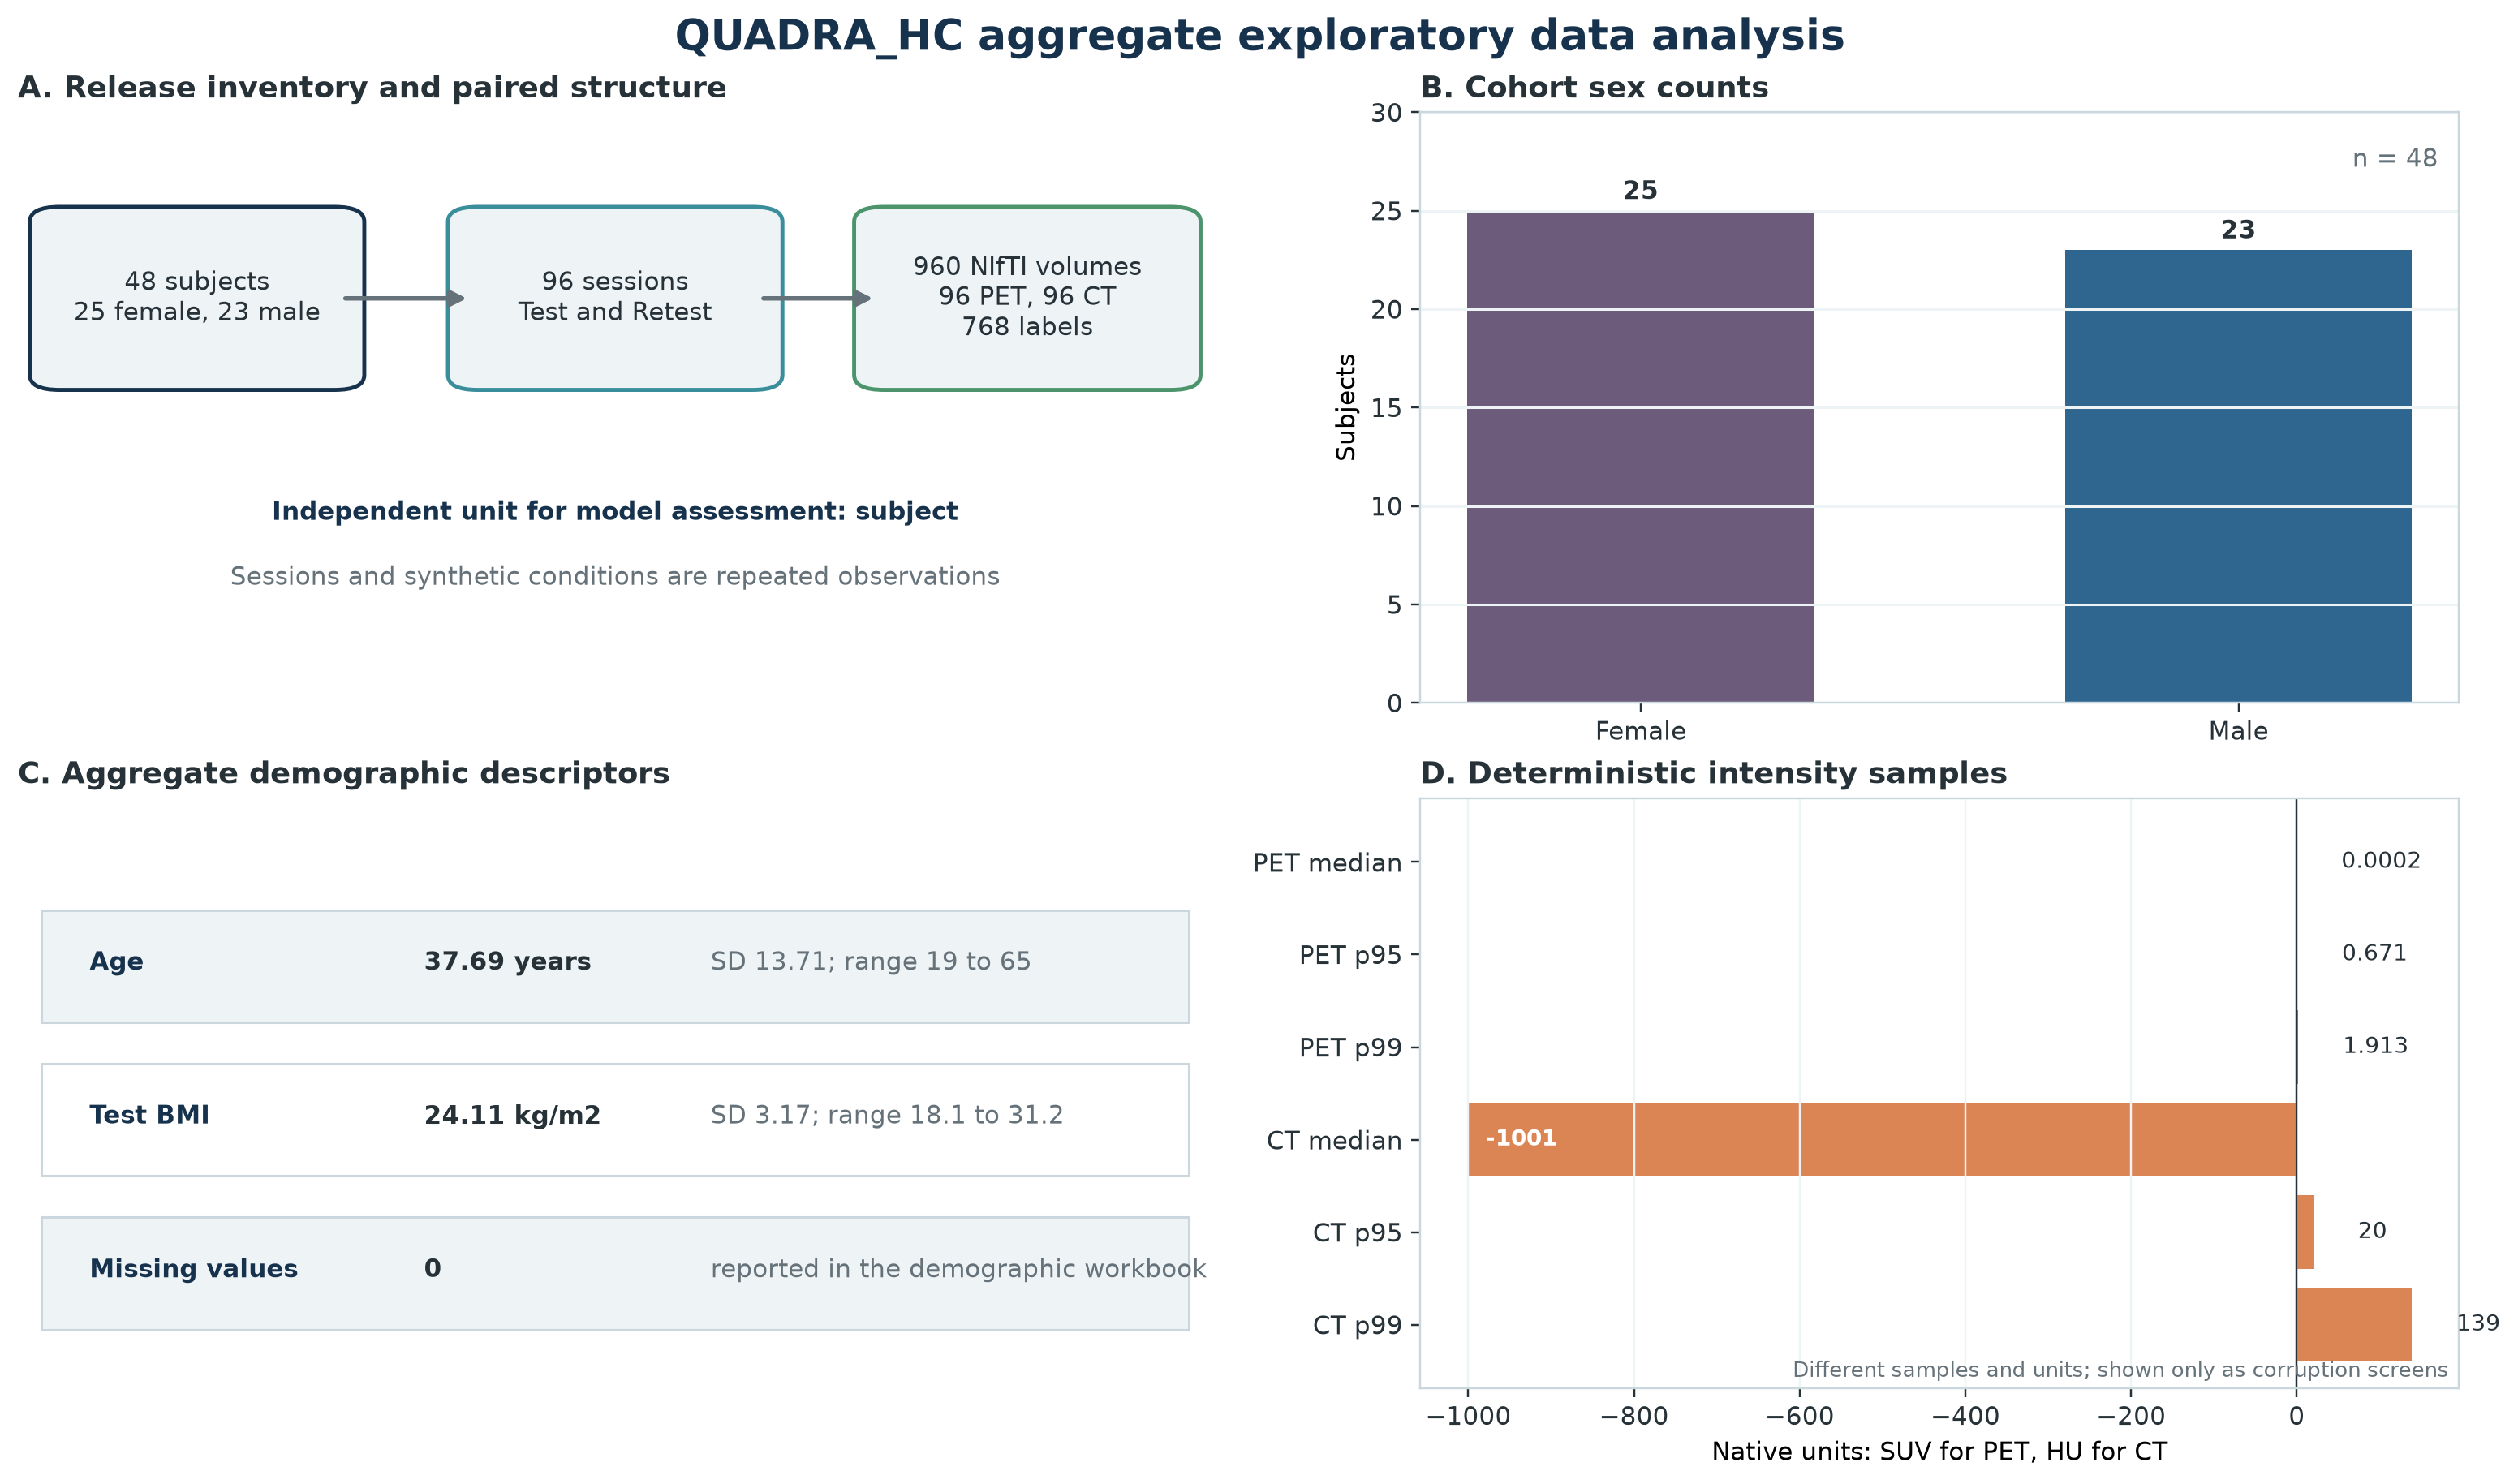
\includegraphics[width=0.99\textwidth]{figures/01_cohort_eda.png}
\caption{Aggregate exploratory data analysis. Population: 48 subjects and 96 paired sessions. Units: counts, years, kg/m$^2$, SUV, and HU as labeled. PET intensity values came from 1,628,736 deterministically sampled voxels across 12 subjects and both visits; CT values came from 544,544 sampled voxels across four subjects and both visits. These samples are corruption screens, not corridor-specific biological distributions, and PET and CT values should not be compared on one numerical scale.}
\label{fig:cohort-eda}
\end{figure}

\subsection{Demographic and acquisition descriptors}

The historical workbook audit reported mean age 37.69 years with SD 13.71 and a local range of 19 to 65. Mean Test BMI was 24.11 kg/m$^2$ with SD 3.17 and range 18.1 to 31.2. These values describe the available cohort. They do not establish representativeness for a broader population or for post-intervention vascular imaging.

The workbook field \texttt{Scan [d]} had a reported median of 35 days, mean 38.75 days, and range 22 to 98 days. The field is interpreted as the Test to Retest interval, but no data dictionary was independently verified. The article reports an average interval of 38 $\pm$ 10 days and a range of 22 to 98 days, which supports that interpretation \citep{quadra2025}. Those article values are frozen in ledger record \evidenceid{SRC-QUADRA-ARTICLE}. Mean injected activity was historically reported as 109.03 MBq at Test and 111.47 MBq at Retest. These are acquisition descriptors, not PET repeatability results.

\begin{figure}[H]
\centering
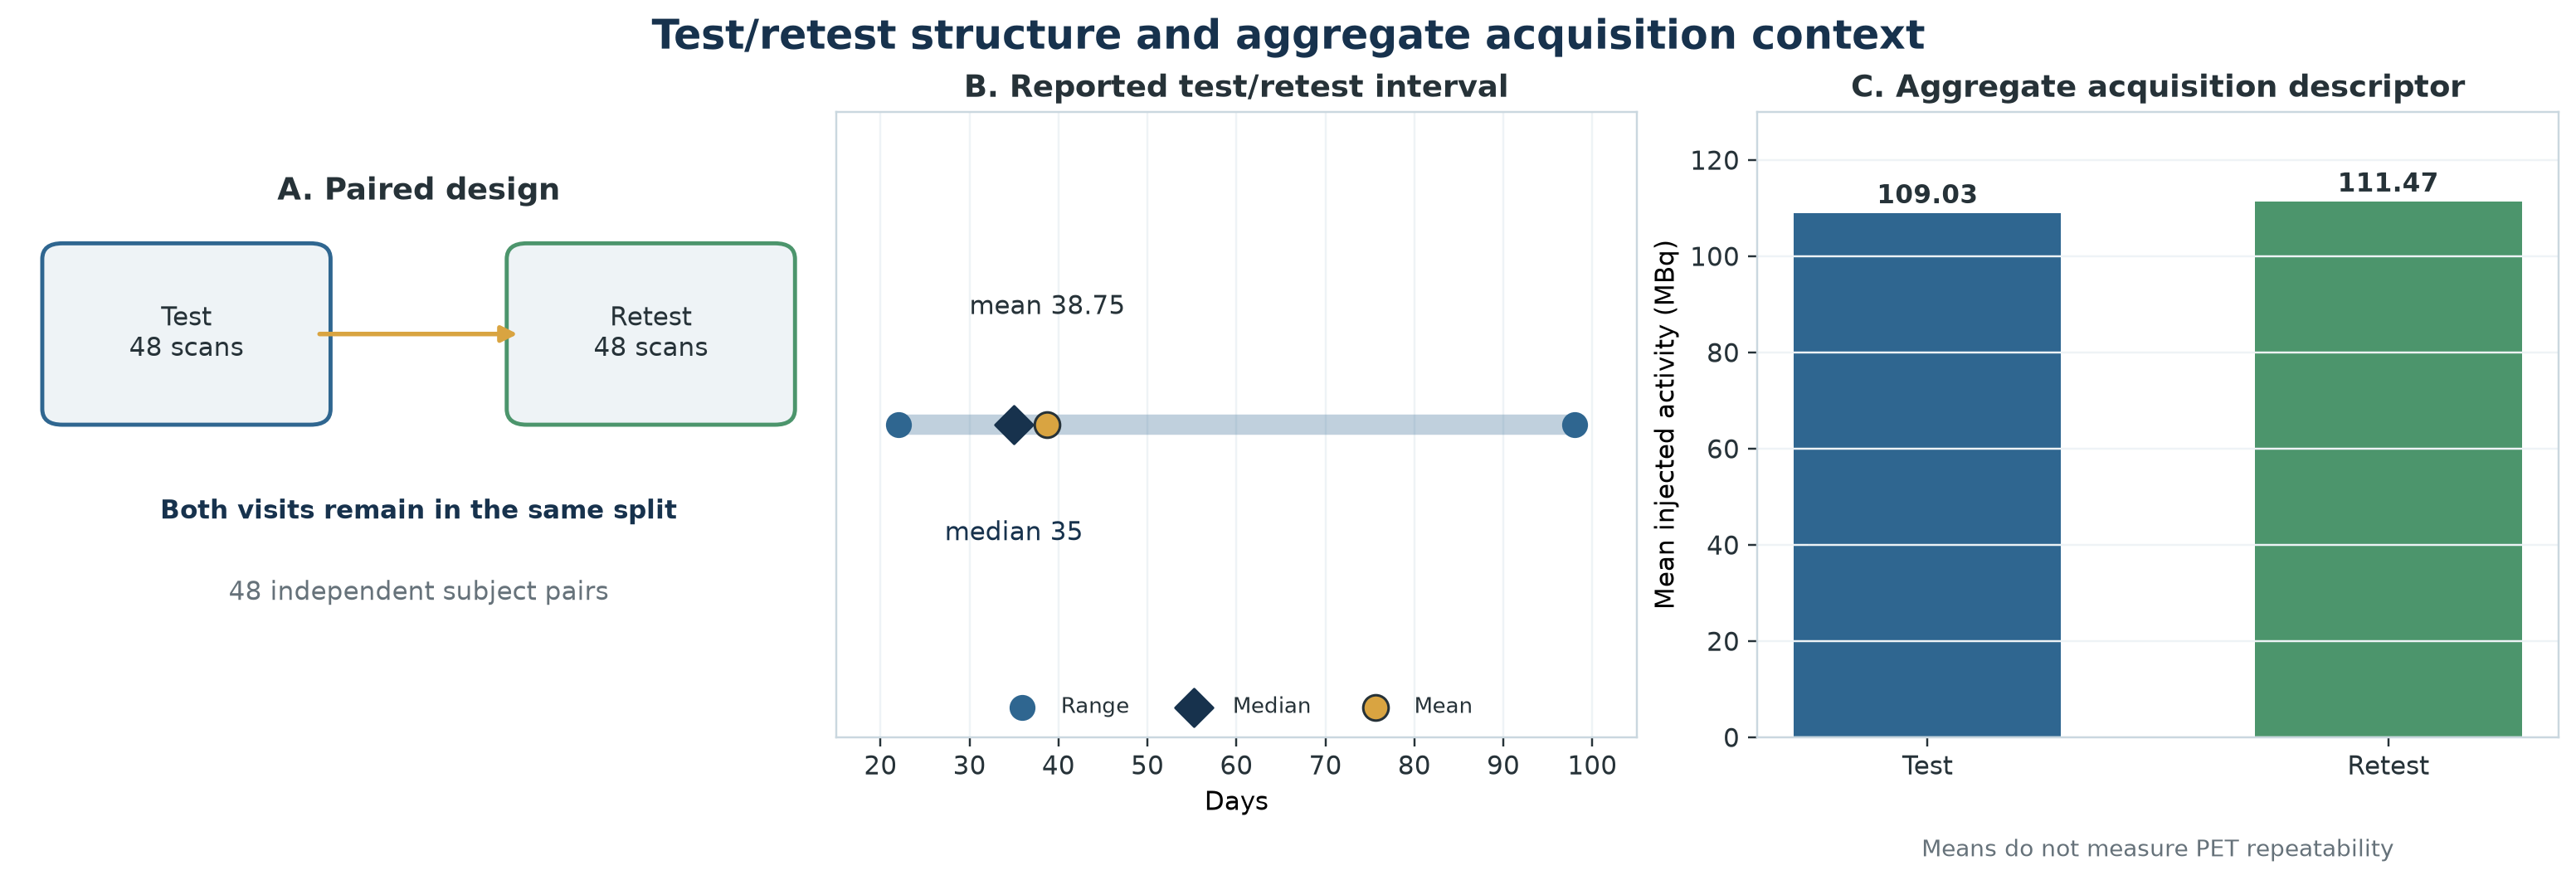
\includegraphics[width=0.99\textwidth]{figures/02_test_retest_summary.png}
\caption{Test/retest structure and acquisition context. Population: 48 paired subjects. Unit: scan count, days, and MBq. The interval range and aggregate injected-activity means summarize source metadata. They do not measure repeatability of SUV, masks, activation, or model scores. Both visits from one subject must remain in the same data partition.}
\label{fig:test-retest}
\end{figure}

\subsection{Image grids and intensity screens}

PET and CT do not use the same array grid. PET has shape $440 \times 440 \times 531$ and spacing $1.65 \times 1.65 \times 2.0$ mm. CT has shape $512 \times 512 \times 531$ and spacing approximately $1.523438 \times 1.523438 \times 2.0$ mm. The article independently reports these reconstruction matrices and spacings \citep{quadra2025}. Historical header checks described both modalities as LAS-oriented, all inspected affines as finite and invertible, and all label grids as matching CT.

The PET physical bounding box lay inside the CT physical bounding box in all 96 sessions in the historical audit. The PET-to-CT physical-volume ratio was 86.6331\%. Bounding-box consistency is necessary but not sufficient. It does not prove that every soft-tissue boundary is locally aligned.

The deterministic PET sample had median 0.0002 SUV, 95th percentile 0.671 SUV, 99th percentile 1.913 SUV, and maximum 192.20 SUV. A total of 0.0915\% of sampled PET values exceeded SUV 10. The CT sample had median -1001 HU, 95th percentile 20 HU, 99th percentile 139 HU, and maximum 2072 HU. Whole-body sampling includes air and physiologic high-uptake regions, so these values cannot define a vascular decision threshold. They support separate network normalization and retention of raw SUV for measurement.

\subsection{Iliac corridor fitness}

The current public MOOSE model inventory lists \texttt{iliac\_artery\_left} and \texttt{iliac\_artery\_right} as labels 7 and 8 in the cardiac model \citep{moose}. The QUADRA article states that release segmentations were generated with MOOSE 3.0.13 \citep{quadra2025}. The public-source values are frozen in ledger records \evidenceid{SRC-MOOSE} and \evidenceid{SRC-QUADRA-ARTICLE}. The local segmentation files did not embed enough version text or an explicit label table to independently bind the archive-era integer mapping. The local mapping is therefore provisional, even though the current public inventory corroborates it.

Under that provisional mapping, historical aggregate checks found both iliac labels nonempty in all 96 sessions. Median left-label size was 2,844 voxels, with range 1,169 to 9,405. Median right-label size was 3,371 voxels, with range 1,107 to 8,355. Only 53 of 96 left masks and 72 of 96 right masks formed one connected component. A conservative bilateral axial-span proxy passed both sides in 84 of 96 sessions. These results support an iliac crop anchor with explicit connectivity and branch-selection QC. They do not establish wall segmentation or exact vessel-boundary accuracy.

\begin{table}[H]
\centering
\caption{Historical corridor fitness. Population: 96 sessions. Unit: voxels or sessions. Limitation: label semantics are provisional and connected-component counts do not resolve anatomical branch choice.}
\label{tab:corridor}
\begin{tabularx}{\textwidth}{lrrX}
\toprule
Measure & Left & Right & Interpretation \\
\midrule
Nonempty label & 96/96 & 96/96 & Presence gate passed under the provisional mapping \\
Median voxels & 2,844 & 3,371 & Adequate aggregate anchor size \\
Voxel range & 1,169 to 9,405 & 1,107 to 8,355 & Substantial session variation \\
One connected component & 53/96 & 72/96 & Branch and fragmentation QC remains necessary \\
\bottomrule
\end{tabularx}
\end{table}

\subsection{Subject-grouped split and realized validation subset}

The intended subject split uses seed 20260713 with sex stratification: 32 training subjects, 8 validation subjects, and 8 test subjects. Historical leakage checks reported disjoint subject partitions, full coverage, and both sessions assigned to the same partition. The training partition contained 17 female and 15 male subjects; validation and test each contained four female and four male subjects.

The later B2 cache did not realize all intended validation evidence. It contained 13 bundles and seven subject clusters after five QC-flagged bundles were excluded from the supersampling-5 cache. Its 208 center slices comprised 78 positive and 130 negative observations. This difference between the planned eight-subject validation partition and the realized seven-cluster cache is material. All B2 results are labeled exploratory.

\section{Physical-coordinate geometry and crop construction}

\subsection{PET as the quantitative reference grid}

PET SUVbw is the quantitative reference grid. The NIfTI affine maps voxel indices into patient-world coordinates, and orientation must be interpreted through that affine rather than through display order \citep{nibabelOrientation,nibabelCoordinates}. CT is resampled to PET with linear interpolation. Masks are resampled with nearest-neighbor interpolation to preserve label identities. A resampler must name the mapping direction because output locations are mapped into the input image \citep{simpleitkResample}.

Canonicalization is a one-time, recorded transform. A correct pipeline retains named forward and inverse mappings between original PET voxels, canonical PET voxels, and crop voxels. An array flip is not a patient-space reflection. Laterality and contralateral sampling must use physical coordinates.

\begin{figure}[H]
\centering
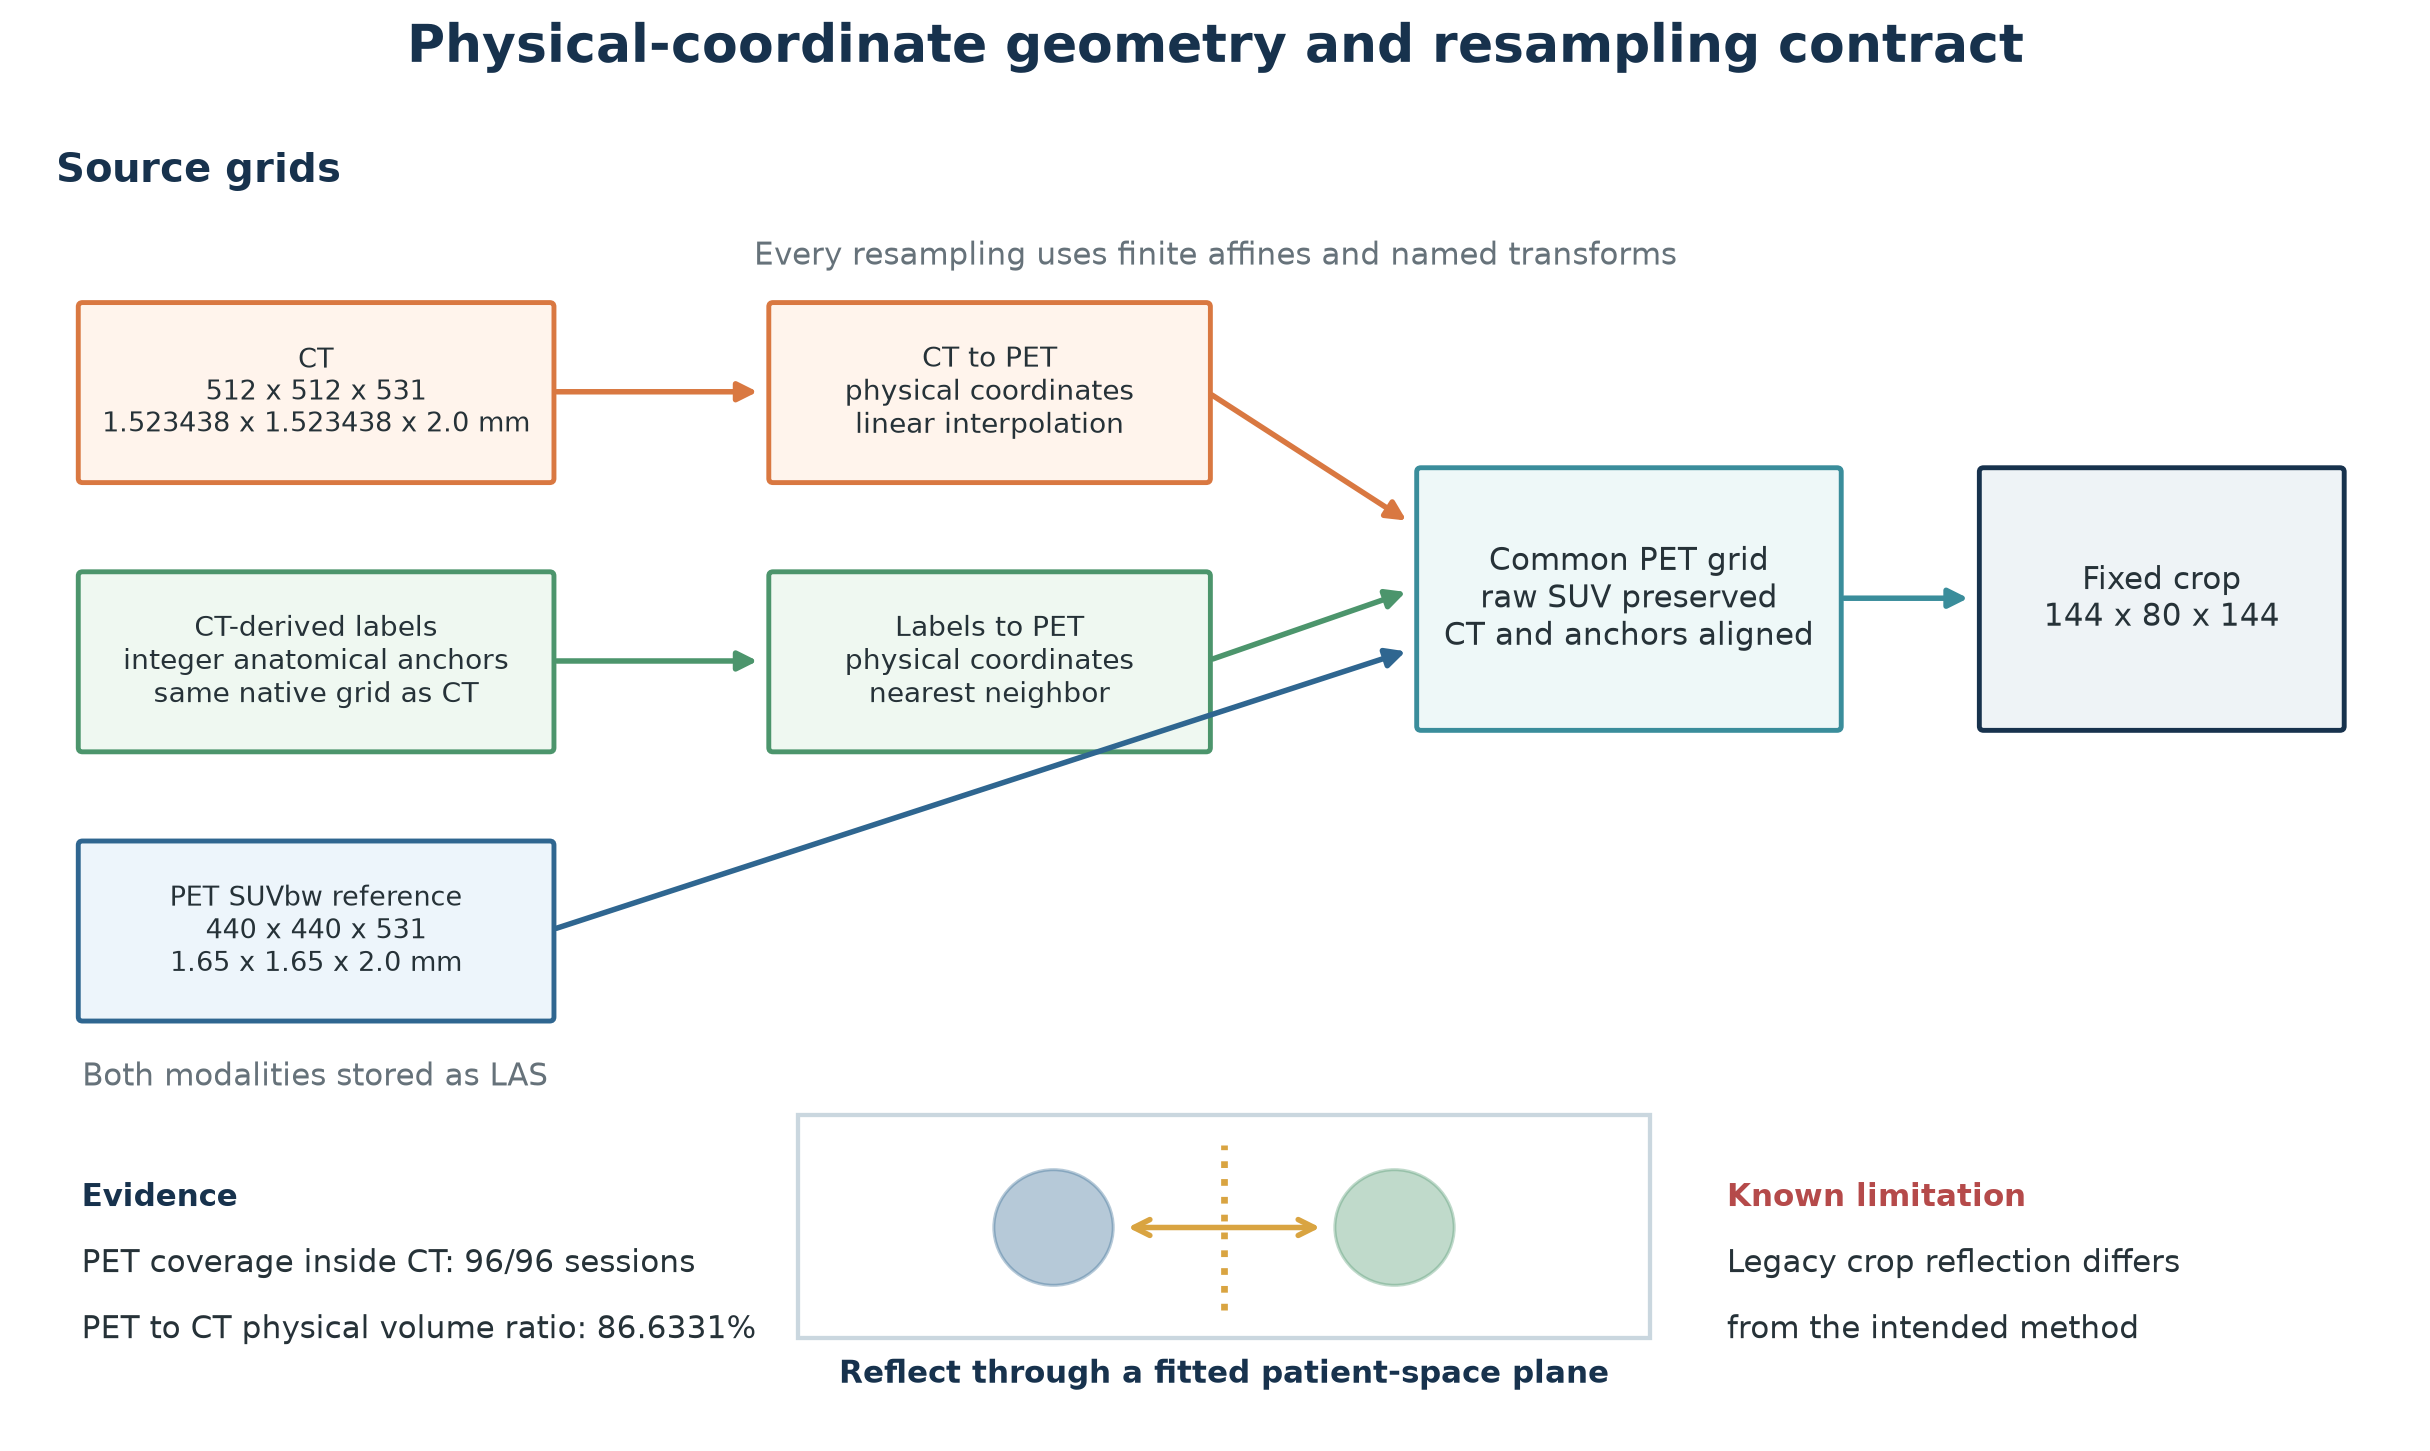
\includegraphics[width=0.99\textwidth]{figures/03_geometry_and_resampling.png}
\caption{Physical-coordinate grid handling. Population: the 96-session aggregate geometry audit. Units: voxels, millimeters, sessions, and percent physical volume. CT values are linearly resampled and labels are nearest-neighbor resampled into the PET SUVbw grid. The diagram is schematic and contains no medical image. Global grid validity and bounding-box overlap do not prove local anatomical alignment.}
\label{fig:geometry}
\end{figure}

\subsection{Crop size decision}

The historical full-cohort corridor audit reported median iliac-only bounding-box dimensions of approximately $153.9 \times 57.9 \times 186.0$ mm. With a 15 mm margin, the largest observed PET-grid crop requirement was $129 \times 70 \times 131$ voxels. The fixed $144 \times 80 \times 144$ crop adds engineering headroom and remains divisible by powers of two used in the network. It is not derived from a measured scanner point-spread function and is not a general scanner specification.

A six-session end-to-end crop receipt produced the fixed shape for all six sessions. Minimum and mean valid-PET coverage were 1.0, none exceeded the crop bounds, reflection residuals ranged from 2.10 to 6.76 mm, and six of six bundle integrity hashes passed. This receipt proves that the implementation ran on a small historical sample. It is not a full-cohort crop acceptance result.

\subsection{Legacy reflection mismatch}

The current crop implementation and the intended reflection contract differ. The current path pairs iliac and femur information per axial slice, forms a plain mean left-to-right normal, and uses the mean of paired midpoints. The intended path uses iliac-only centerlines, pairs points at normalized arc-length locations over a shared usable extent, orients each pair toward patient RAS right, computes a resistant mean normal, and uses a median plane offset.

The reflection method affects the contralateral network view, the PET difference channel, the source baseline, laterality, and quantitative ratios. The current crops remain useful for exploratory development, but native-space evaluation and product quantification should not be promoted until the crop bundles are regenerated under one reconciled method and the old bundles are rejected by schema version.

\section{Synthetic-source simulation}

\subsection{Image-domain source equation}

The simulator inserts one source into an already validated PET grid:

\begin{equation}
\mathrm{PET}_{\mathrm{syn}} = \mathrm{PET}_{\mathrm{orig}} + G_{\sigma} * \left[(m-1) B F H\right].
\label{eq:simulation}
\end{equation}

Here, $B$ is a contralateral background estimate, $m$ is the nominal pre-blur uptake multiplier, $F$ is the fractional source occupancy, $H$ is a positive low-frequency heterogeneity field, and $G_{\sigma}$ is a unit-sum Gaussian image-blur operator applied only to the synthetic excess. The current implementation uses a 20\%-per-tail trimmed mean for $B$ and requires a positive, finite result from enough contralateral samples.

Fractional occupancy is computed by physical supersampling around a centerline capsule. The default supersampling factor is 5. The current design range is radius 2 to 6 mm and length 45 mm. The supervision mask is $F \geq 0.5$. The heterogeneity parameter is 0.15 and the field is normalized to occupancy-weighted mean 1.

The synthetic excess is blurred with per-axis voxel sigma derived from physical FWHM:

\begin{equation}
\sigma_i = \frac{\mathrm{FWHM}_{\mathrm{mm}}}{2\sqrt{2\ln 2}\,s_i},
\end{equation}

where $s_i$ is voxel spacing along axis $i$. The implementation uses zero-valued constant boundaries and truncation at four standard deviations, consistent with the explicit SciPy filter parameters \citep{scipyGaussian}. The 4 to 8 mm blur settings are controlled image-domain factors. They are not measurements of scanner resolution.

\begin{figure}[H]
\centering
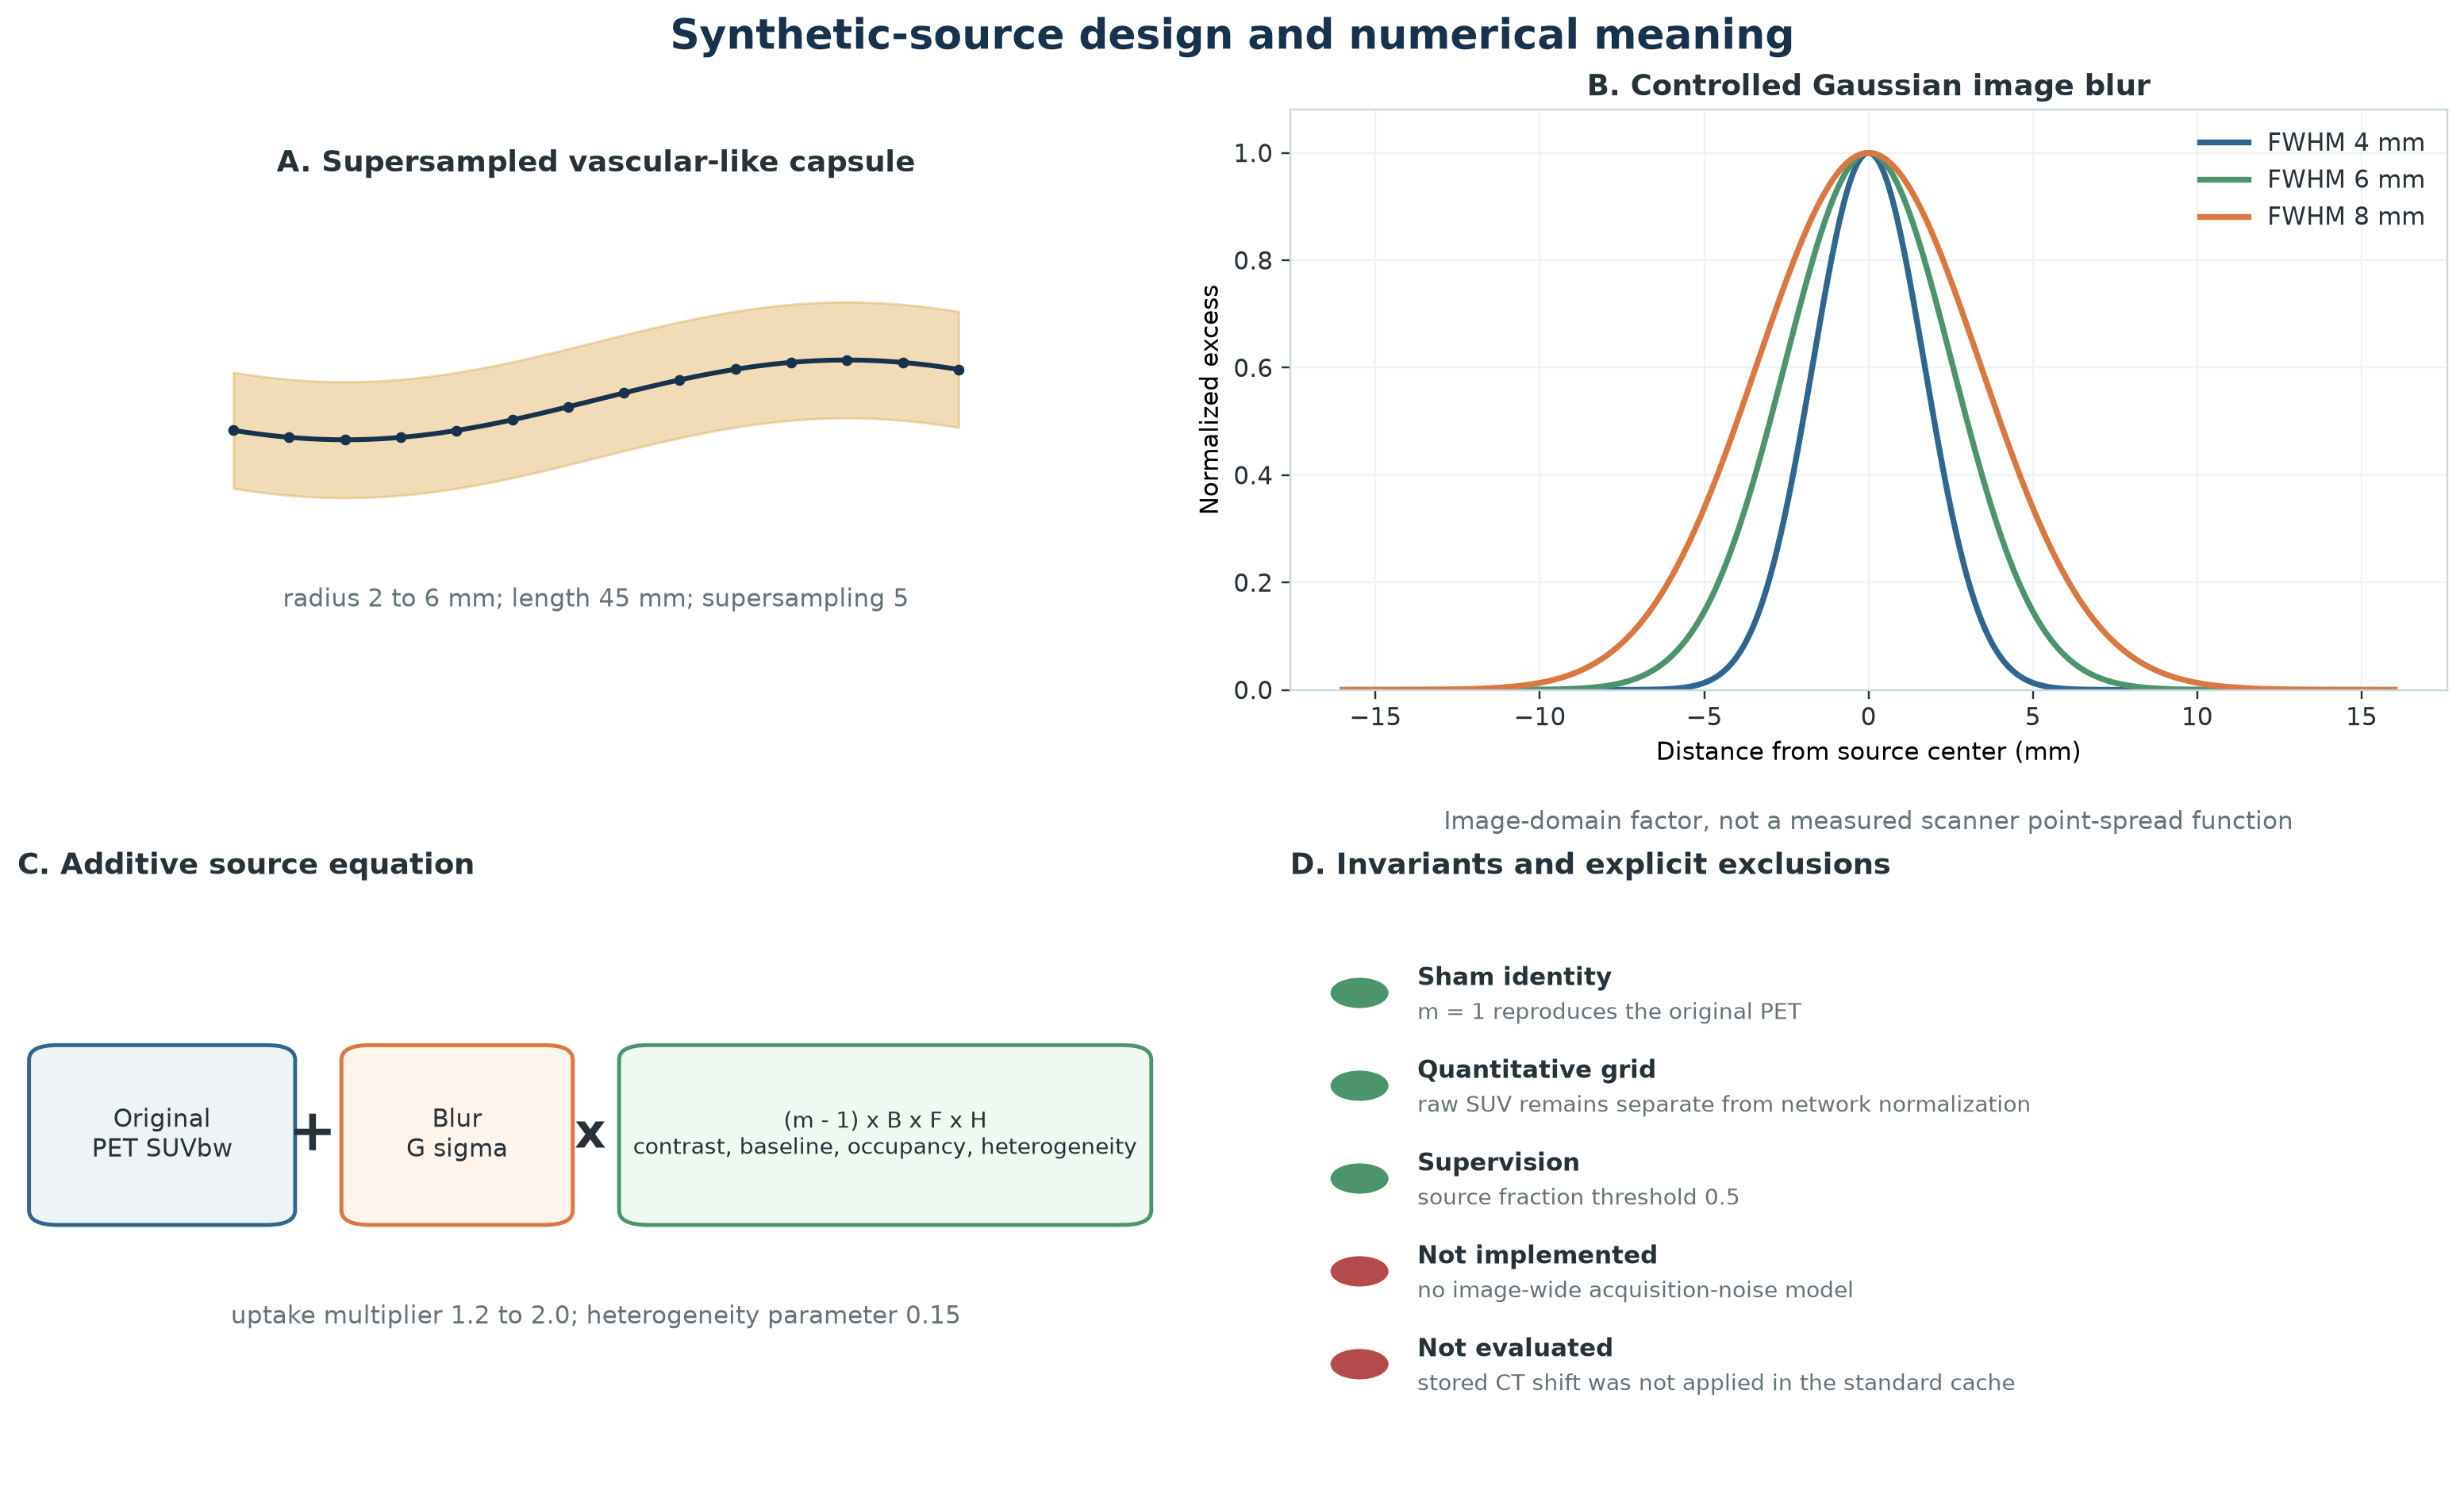
\includegraphics[width=0.99\textwidth]{figures/04_simulation_contract.png}
\caption{Synthetic-source contract. Population: generated sources, not human abnormalities. Units: millimeters and normalized synthetic excess. The capsule and Gaussian curves are schematics generated without medical images. Blur FWHM is an image-domain factor, not a scanner point-spread measurement. The standard cache did not apply the stored CT-shift field, and no image-wide acquisition-noise model was used.}
\label{fig:simulation}
\end{figure}

\subsection{Numerical invariants}

The implemented generator encodes four important checks:

\begin{itemize}
  \item $m=1$ is a sham and should reproduce the input PET within the declared numeric tolerance.
  \item The synthetic excess is nonnegative for the supported multiplier range.
  \item Rasterized capsule volume is compared with its analytic volume under generated fixtures.
  \item Activity conservation and recovered blur width are checked when the source has a complete four-sigma margin.
\end{itemize}

These are implementation tests, not evidence that the synthetic source matches a biological lesion or a scanner reconstruction process.

\subsection{Network copies and quantitative copies}

The network PET copy is clipped to 0 to 10 SUV and divided by 10. The CT copy is clipped to -1000 to 1000 HU and divided by 1000. Raw SUVbw remains separate. A clipped tensor serves network conditioning, whereas quantitative PET reporting requires the separate raw SUVbw copy. The historical PET sample found 0.0915\% of sampled values above SUV 10, which confirms the need to keep the quantitative copy separate.

\subsection{Factors that were not evaluated}

The standard cache carried a CT-shift field in simulation metadata, but that shift was not applied to the CT input. No result involving that field is reported. The simulator also does not add image-wide acquisition noise. The later texture-proxy analysis describes the observed raw-PET background. It is not an acquisition simulation. A future registration stress must move only the CT input while PET and labels remain fixed, with a verified transform and balanced direction assignment.

\section{Transparent threshold baseline}

\subsection{Implemented behavior}

The threshold module provides two transparent score maps: bilateral positive excess and raw SUV. It thresholds the selected map, labels 3D components with 26-connectivity, matches components to one synthetic target, computes an F2 summary, and can freeze a validation threshold under an untouched-scan component ceiling. This is useful because a learned method should be compared with a rule whose behavior can be inspected directly.

\subsection{Contract gaps}

The current standalone baseline is not fully promotion compliant. Its positive-case F2 path counts unmatched components within positive images, while the intended promotion contract defines the negative contribution using sham and untouched scans with any activation. Minimum physical component volume is absent, so the corresponding tie rule is also absent. The toy $8 \times 32 \times 32$ reference experiment uses fabricated data and a different detection rule. It must remain separate from the learned-model atlas.

Table~\ref{tab:baseline-gap} distinguishes what is implemented from what is required for a final comparison.

\begin{table}[H]
\centering
\caption{Threshold baseline status. Population: implementation interfaces and generated-fixture tests. Unit: rule. Limitation: no promotion-compliant aggregate comparison has been verified.}
\label{tab:baseline-gap}
\begin{tabularx}{\textwidth}{>{\bfseries}p{0.23\textwidth} X X}
\toprule
Element & Current path & Required final path \\
\midrule
Score map & Positive mirrored excess or raw SUV & Freeze one declared score map before sealed test access \\
Components & 26-connectivity & 26-connectivity plus minimum physical volume \\
Positive matching & Target intersection with deterministic component handling & Retain frozen tie order and all unmatched components \\
Negative term & Separate ceiling plus a narrower positive-case error count & Sham and untouched scan activation in the frozen F2 definition \\
Threshold choice & Validation sweep with infeasible result supported & Freeze threshold, volume, and score rule once \\
Promotion evidence & Not verified & Compare on one validation decision under the same scan-level definitions \\
\bottomrule
\end{tabularx}
\end{table}

\section{Learned model and training pipeline}

\subsection{2.5D bilateral tensor contract}

Each center-slice sample contains two views. The direct view has five adjacent PET slices followed by five adjacent CT slices. The reflected view has the same channel layout after physical reflection. A separate five-channel PET difference tensor preserves a full-resolution bilateral cue. The center slice supplies the target and valid-region masks.

Five adjacent slices span 8 mm from first to last center in the source PET spacing. This is an engineering choice within a 2.5D model. It does not capture the entire 45 mm source at once. Scan-level output therefore requires deterministic slicing, stitching, native-grid reconstruction, and 3D component analysis.

\subsection{Shared-weight Siamese U-Net}

The architecture follows a shared-branch comparison design \citep{siamese2015} with a U-Net-style encoder and decoder \citep{unet2015}. One encoder instance is applied to both views, so left and reflected inputs are processed with the same parameters. At each scale, left features, right features, and their absolute difference are concatenated and projected with a $1 \times 1$ convolution. The decoder receives fused skip features and the full-resolution difference stem.

GroupNorm is used instead of batch-dependent normalization \citep{groupnorm2018}. GELU supplies the activation. The B2 configuration adds training-only auxiliary heads at downsampling factors 2 and 4, with weights 0.5 and 0.25. The inference output remains one full-resolution center-slice logit map. The sigmoid map is reported only as an uncalibrated \scoreterm.

\begin{figure}[H]
\centering
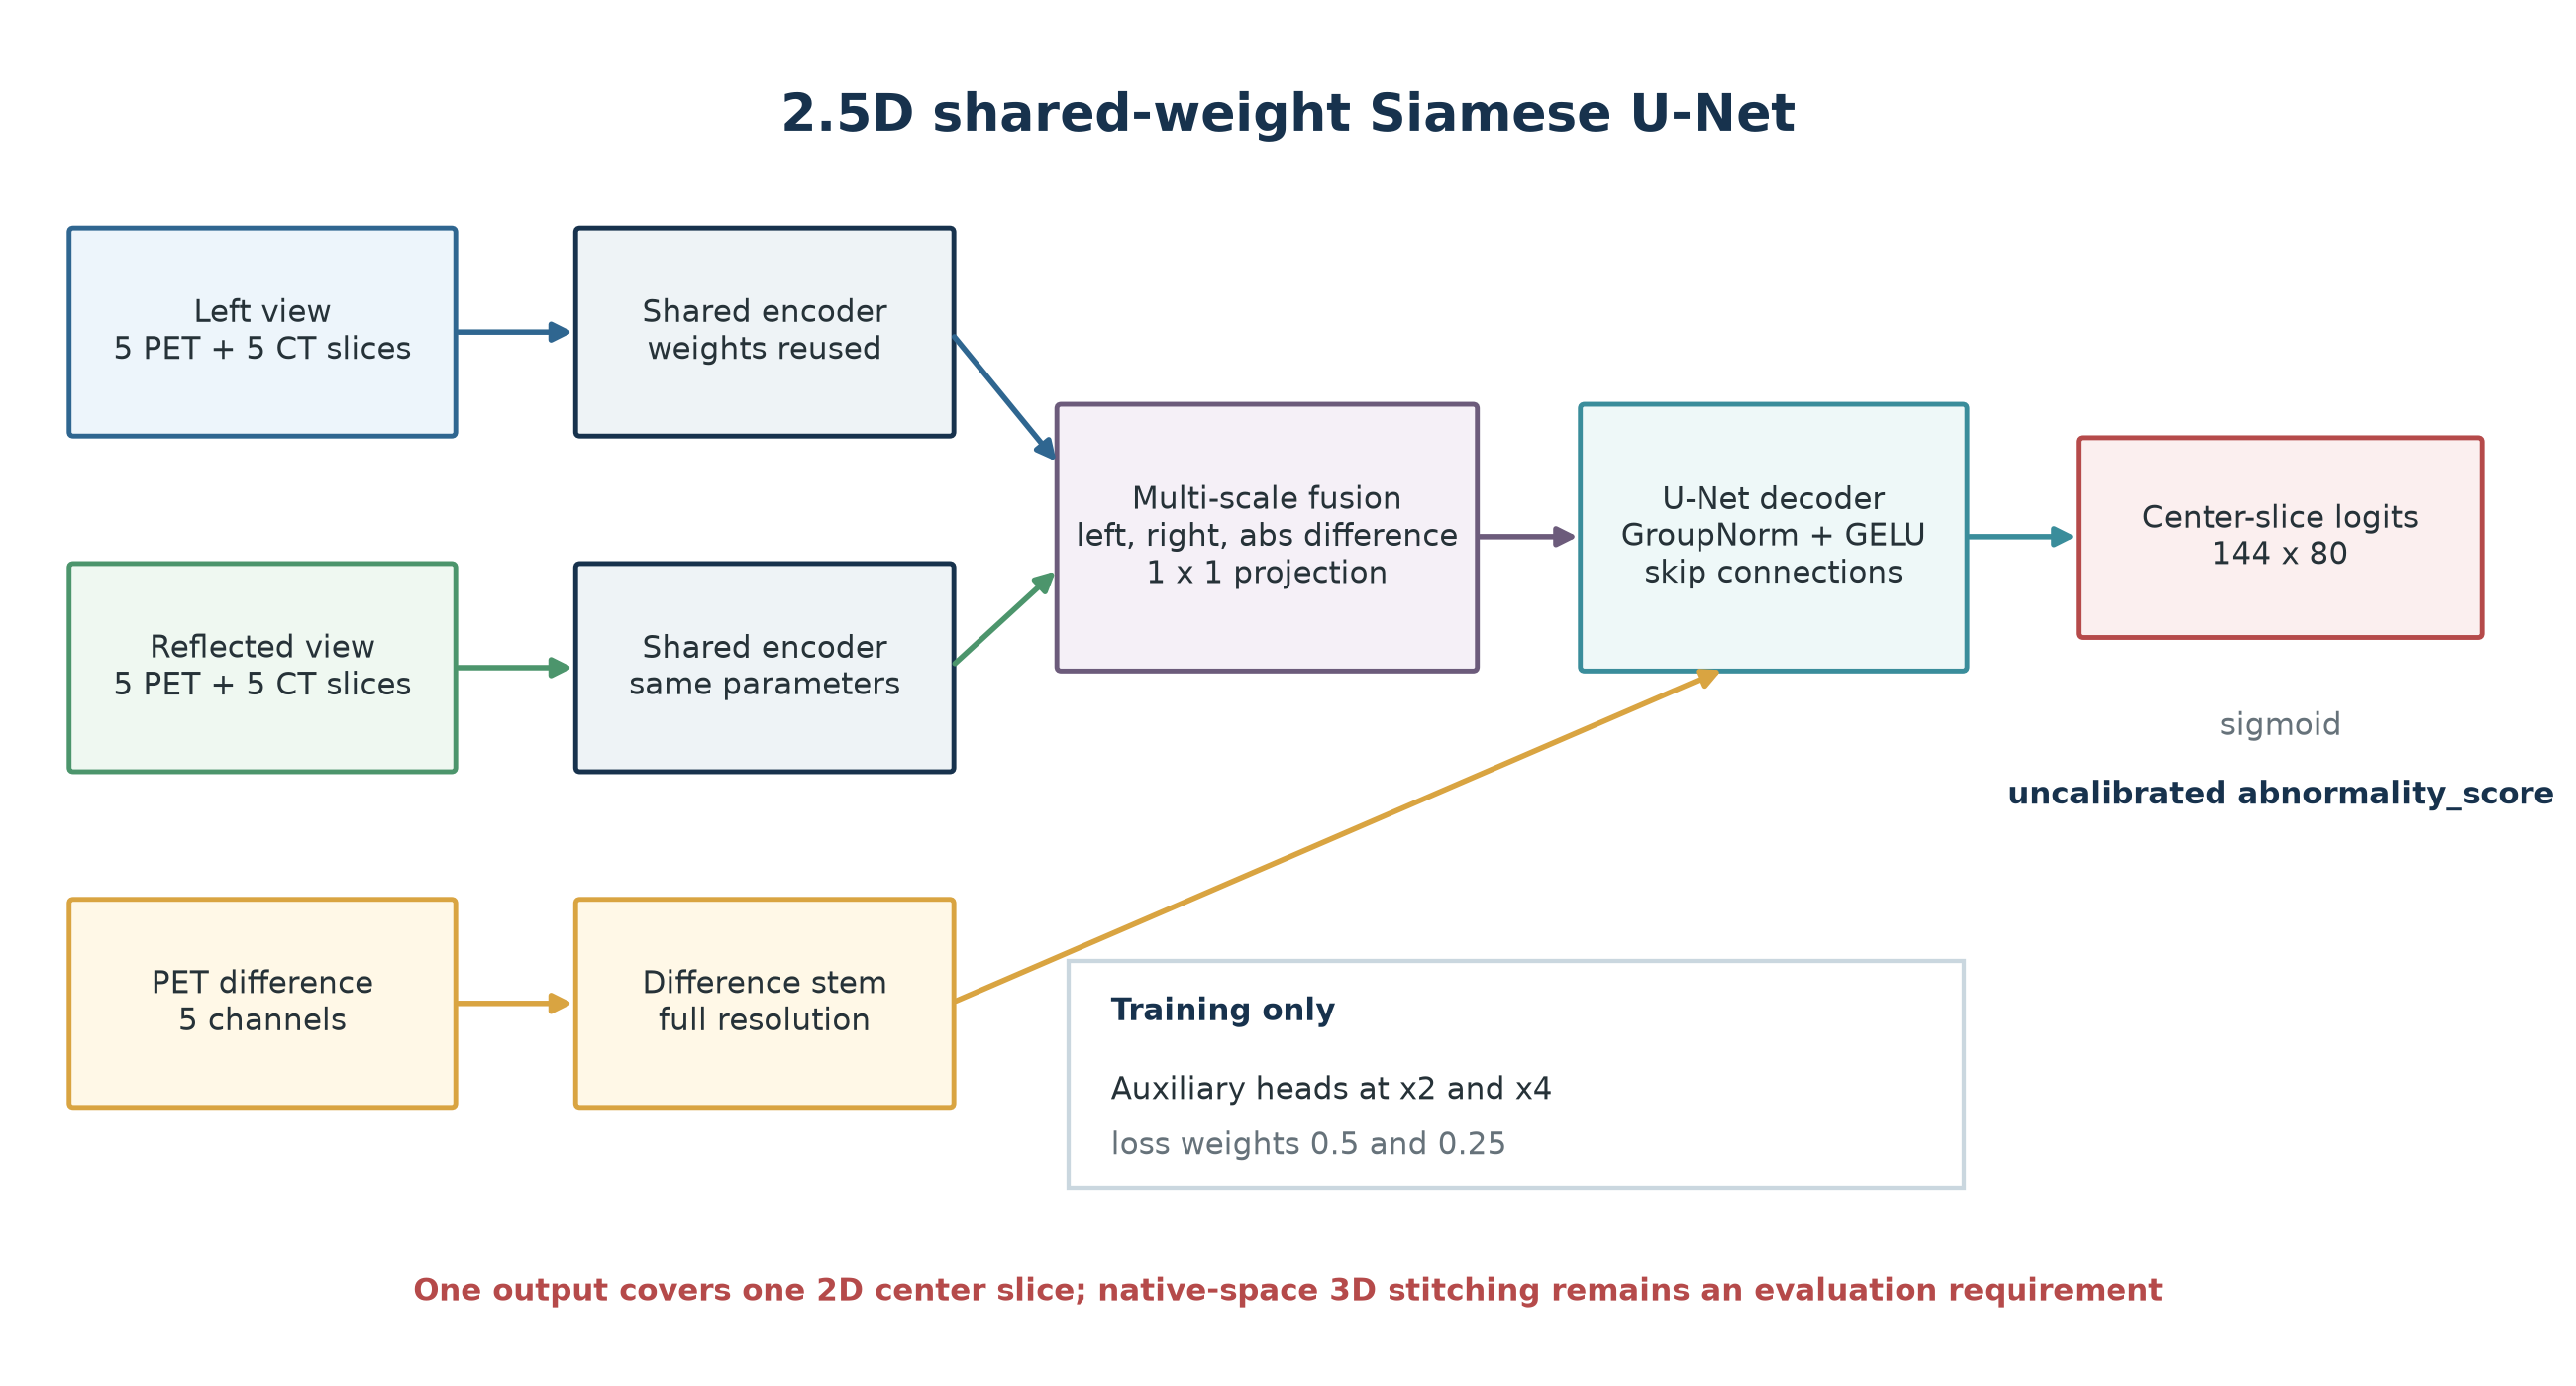
\includegraphics[width=0.99\textwidth]{figures/05_model_architecture.png}
\caption{Implemented B2 architecture. Population: model center-slice samples. Unit: channels and output pixels. Each branch has five PET and five CT slices, with five PET-difference channels. The diagram is a code-derived schematic. It does not imply native-space 3D inference, calibration, or clinical interpretation.}
\label{fig:model}
\end{figure}

\subsection{Training configuration and cache}

The primary B2 configuration used seed 20260716, batch size 128, up to 150 epochs, CUDA automatic mixed precision, geometric and intensity augmentation, exponential moving average decay 0.999, hard-negative mining, and deep supervision. Checkpoint selection required component precision at least 0.901 and component F1 at least 0.859 before maximizing positive IoU. A second configured seed was 20260722, but this report does not claim a formal multi-seed aggregate.

The training cache contained 1,240 center slices. The validation cache contained 208 center slices, of which 78 were positive and 130 were negative. Five QC-flagged bundles were excluded from the supersampling-5 cache. The validation observations came from 13 bundles and seven subject clusters. Loss development included overlap and classification terms; focal Tversky-style objectives were examined to address sparse foregrounds \citep{focaltversky2019}. The report does not infer model quality from training loss alone.

\subsection{Score semantics}

The sigmoid output has not been calibrated against a clinical endpoint or a declared case-level calibration set. It is therefore an \scoreterm, not a calibrated estimate. Threshold 0.5 is an operating point for the exploratory validation cache. It is not a biological threshold or a clinical decision threshold.

\section{Evaluation design and current evidence}

\subsection{Independent unit and current evaluator}

The correct independent unit is the subject. Center slices, visits, bilateral views, seeds, and simulation conditions derived from one subject are correlated. Resampling individual slices as if each represented a new subject would understate uncertainty.

The current historical evaluator operates on 2D center slices. It uses maximal 2D connectivity, which is 8-connectivity, and best-IoU component matching with a threshold of 0.1. It produced subject-clustered intervals for aggregate metrics. These mechanics do not match the intended final evaluator, which requires stitched native-space 3D masks, 26-connectivity, any-intersection source matching under the frozen tie rule, and 5,000 subject-cluster bootstrap replicates. Metric implementation choices matter in sparse segmentation, especially for empty masks and small targets \citep{metricPitfalls2021}.

\subsection{B2 exploratory validation result}

At threshold 0.5 and minimum component size 0 pixels, the B2 checkpoint produced target-overlapping predictions on 75 of 78 positive center slices, or 96.1538\%. Mean positive IoU was 0.614895. Component precision was 0.925926 and component F1 was 0.943396. On 130 negative center slices, 37 had activation and 93 had no activation, giving an activation proportion of 28.4615\% and a clean proportion of 71.5385\%.

These terms are deliberately image-domain terms. The 75 of 78 count is not clinical sensitivity. The 37 of 130 count is not a clinical false-positive rate. The population is a repeated center-slice validation cache in healthy-control backgrounds, not a clinical case series.

\subsection{B0 and B2 aggregate comparison}

The historical B0 mean IoU was 0.596842 and B2 mean IoU was 0.614895, a reported change of 0.0181 with interval 0.0039 to 0.0317. B0 clean rate was 0.692308 and B2 clean rate was 0.715385, a change of 0.0231 whose reported interval included zero. The IoU difference is small in absolute terms. The clean-rate result is directionally favorable but uncertain. Neither comparison substitutes for the missing promotion-compliant threshold baseline or sealed test.

\begin{table}[H]
\centering
\caption{Exploratory B2 validation summary. Population: 208 center slices from 13 bundles and seven subject clusters. Unit: repeated center-slice observation, with subjects retained as the clustering unit in the historical evaluation. Limitation: not sealed test, scan-level, native-space 3D, or clinical evidence.}
\label{tab:b2}
\begin{tabular}{lrr}
\toprule
Measure & Value & Count or context \\
\midrule
Positive mean IoU & 0.614895 & 78 positive center slices \\
Target-overlapping positive slices & 96.1538\% & 75/78 \\
Component precision & 0.925926 & Exploratory component metric \\
Component F1 & 0.943396 & Exploratory component metric \\
Negative-slice activation & 28.4615\% & 37/130 \\
Negative-slice clean proportion & 71.5385\% & 93/130 \\
\bottomrule
\end{tabular}
\end{table}

\section{Descriptive detectability atlas}

\subsection{One-factor strata}

Each positive factor was divided into three equal-count strata of 26 center slices. Radius-stratum target overlap was 92.3\%, 100\%, and 96.2\%, with mean IoU 0.461, 0.687, and 0.697. The smallest-radius stratum had the lowest overlap quality.

Uptake-stratum target overlap was 88.5\%, 100\%, and 100\%, with mean IoU 0.500, 0.718, and 0.627. The middle group exceeded the high group, so a simple monotonic uptake claim is not supported.

Blur-stratum target overlap was 100\%, 100\%, and 88.5\%, with mean IoU 0.707, 0.623, and 0.515. The pattern is consistent with a harder image-domain localization task at higher blur, but it does not identify scanner sensitivity or a clinical resolution threshold.

\subsection{Radius by uptake matrix}

The nine radius-by-uptake cells contain 5 to 12 observations. Mean IoU ranged from 0.429 in the low-radius, low-uptake cell to 0.821 in the high-radius, high-uptake cell. The low-radius row stayed below 0.50 across all uptake strata. Some cells are too small for a precise standalone estimate. The matrix is descriptive and repeated within subjects.

\begin{figure}[H]
\centering
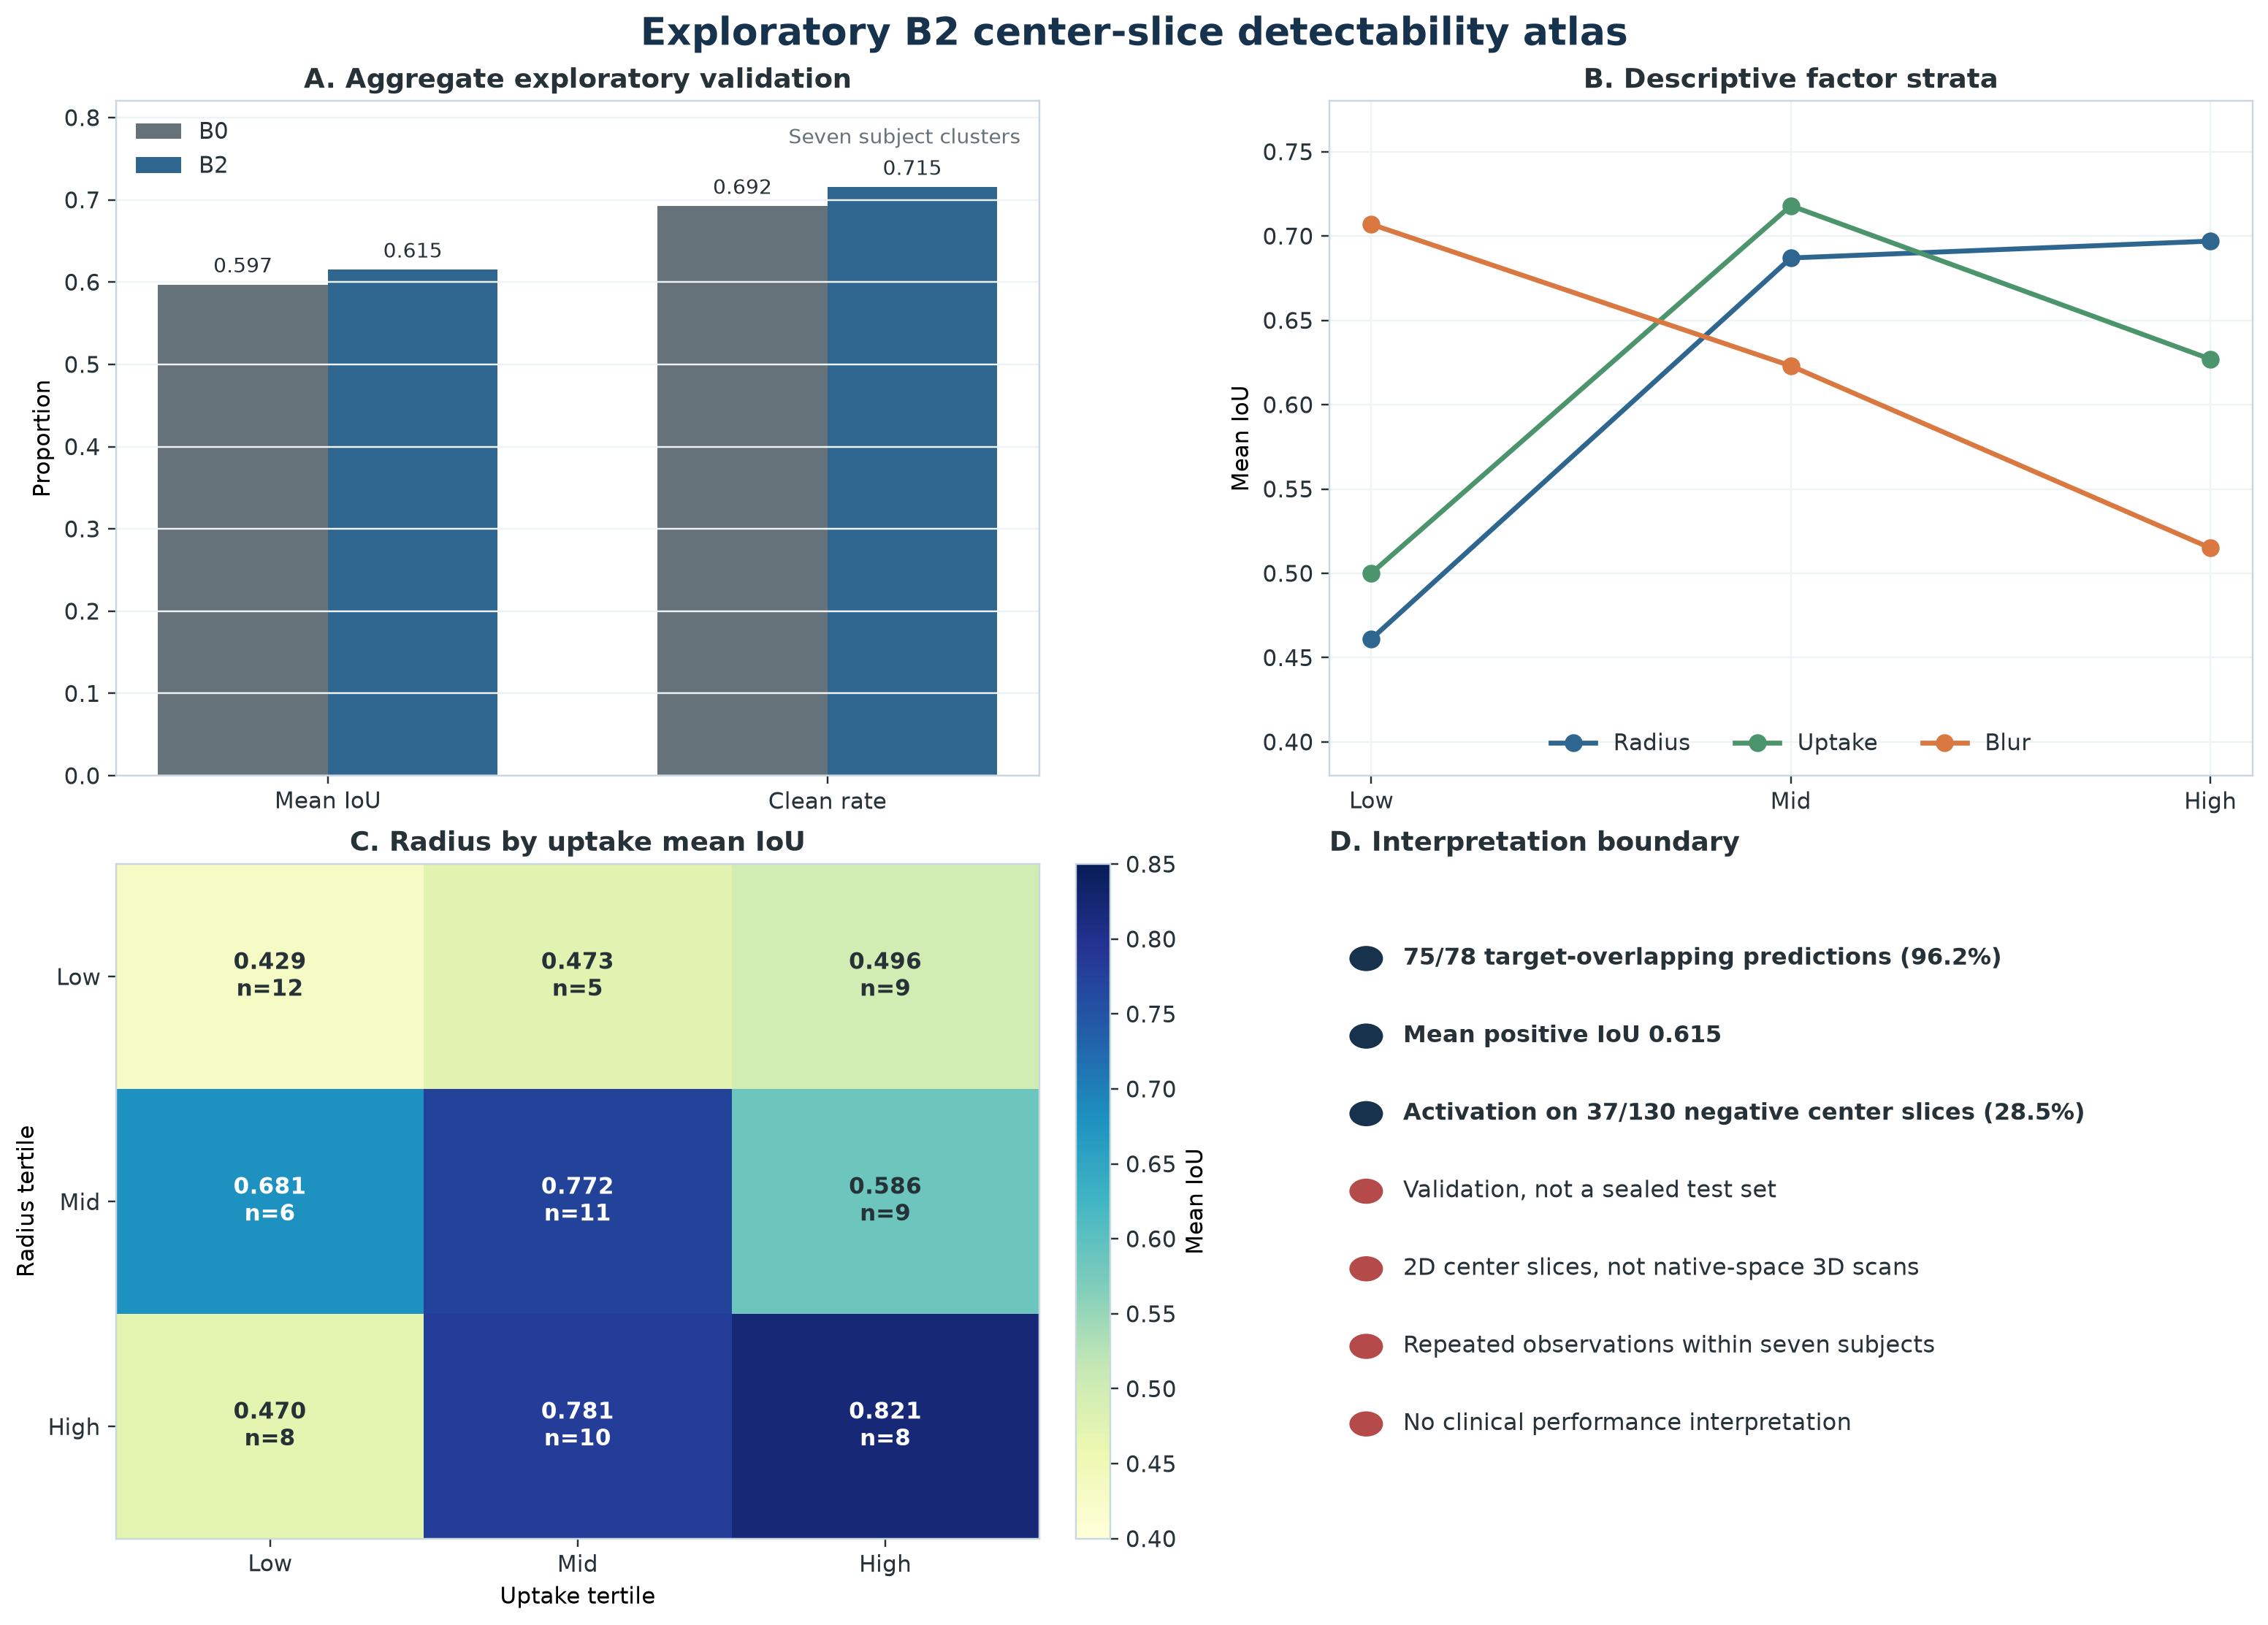
\includegraphics[width=0.99\textwidth]{figures/06_detectability_atlas.png}
\caption{Exploratory B2 detectability atlas. Population: 78 positive and 130 negative validation center slices from seven subject clusters. Units: IoU, proportions, and cell counts. B0 and B2 bars use the same historical validation cache. Factor strata contain repeated observations and the heatmap cells contain only 5 to 12 slices. The figure does not show sealed test, scan-level, native-space 3D, or clinical performance.}
\label{fig:atlas}
\end{figure}

\subsection{Activation by derived raw-PET texture proxy}

The negative validation slices were stratified by a derived raw-PET texture quantity. Activation occurred on 16.1\% of 62 low-stratum slices, 23.1\% of 39 middle-stratum slices, and 62.1\% of 29 high-stratum slices. The direction suggests that complex or variable backgrounds deserve explicit stress testing and error analysis.

The quantity is not an acquisition-noise parameter. It is a summary derived from the observed PET background. The 130 slices are not 130 independent subjects. Confirmatory clustered inference was not completed under the final evaluation contract, so this report does not attach an inferential claim to the gradient.

\begin{figure}[H]
\centering
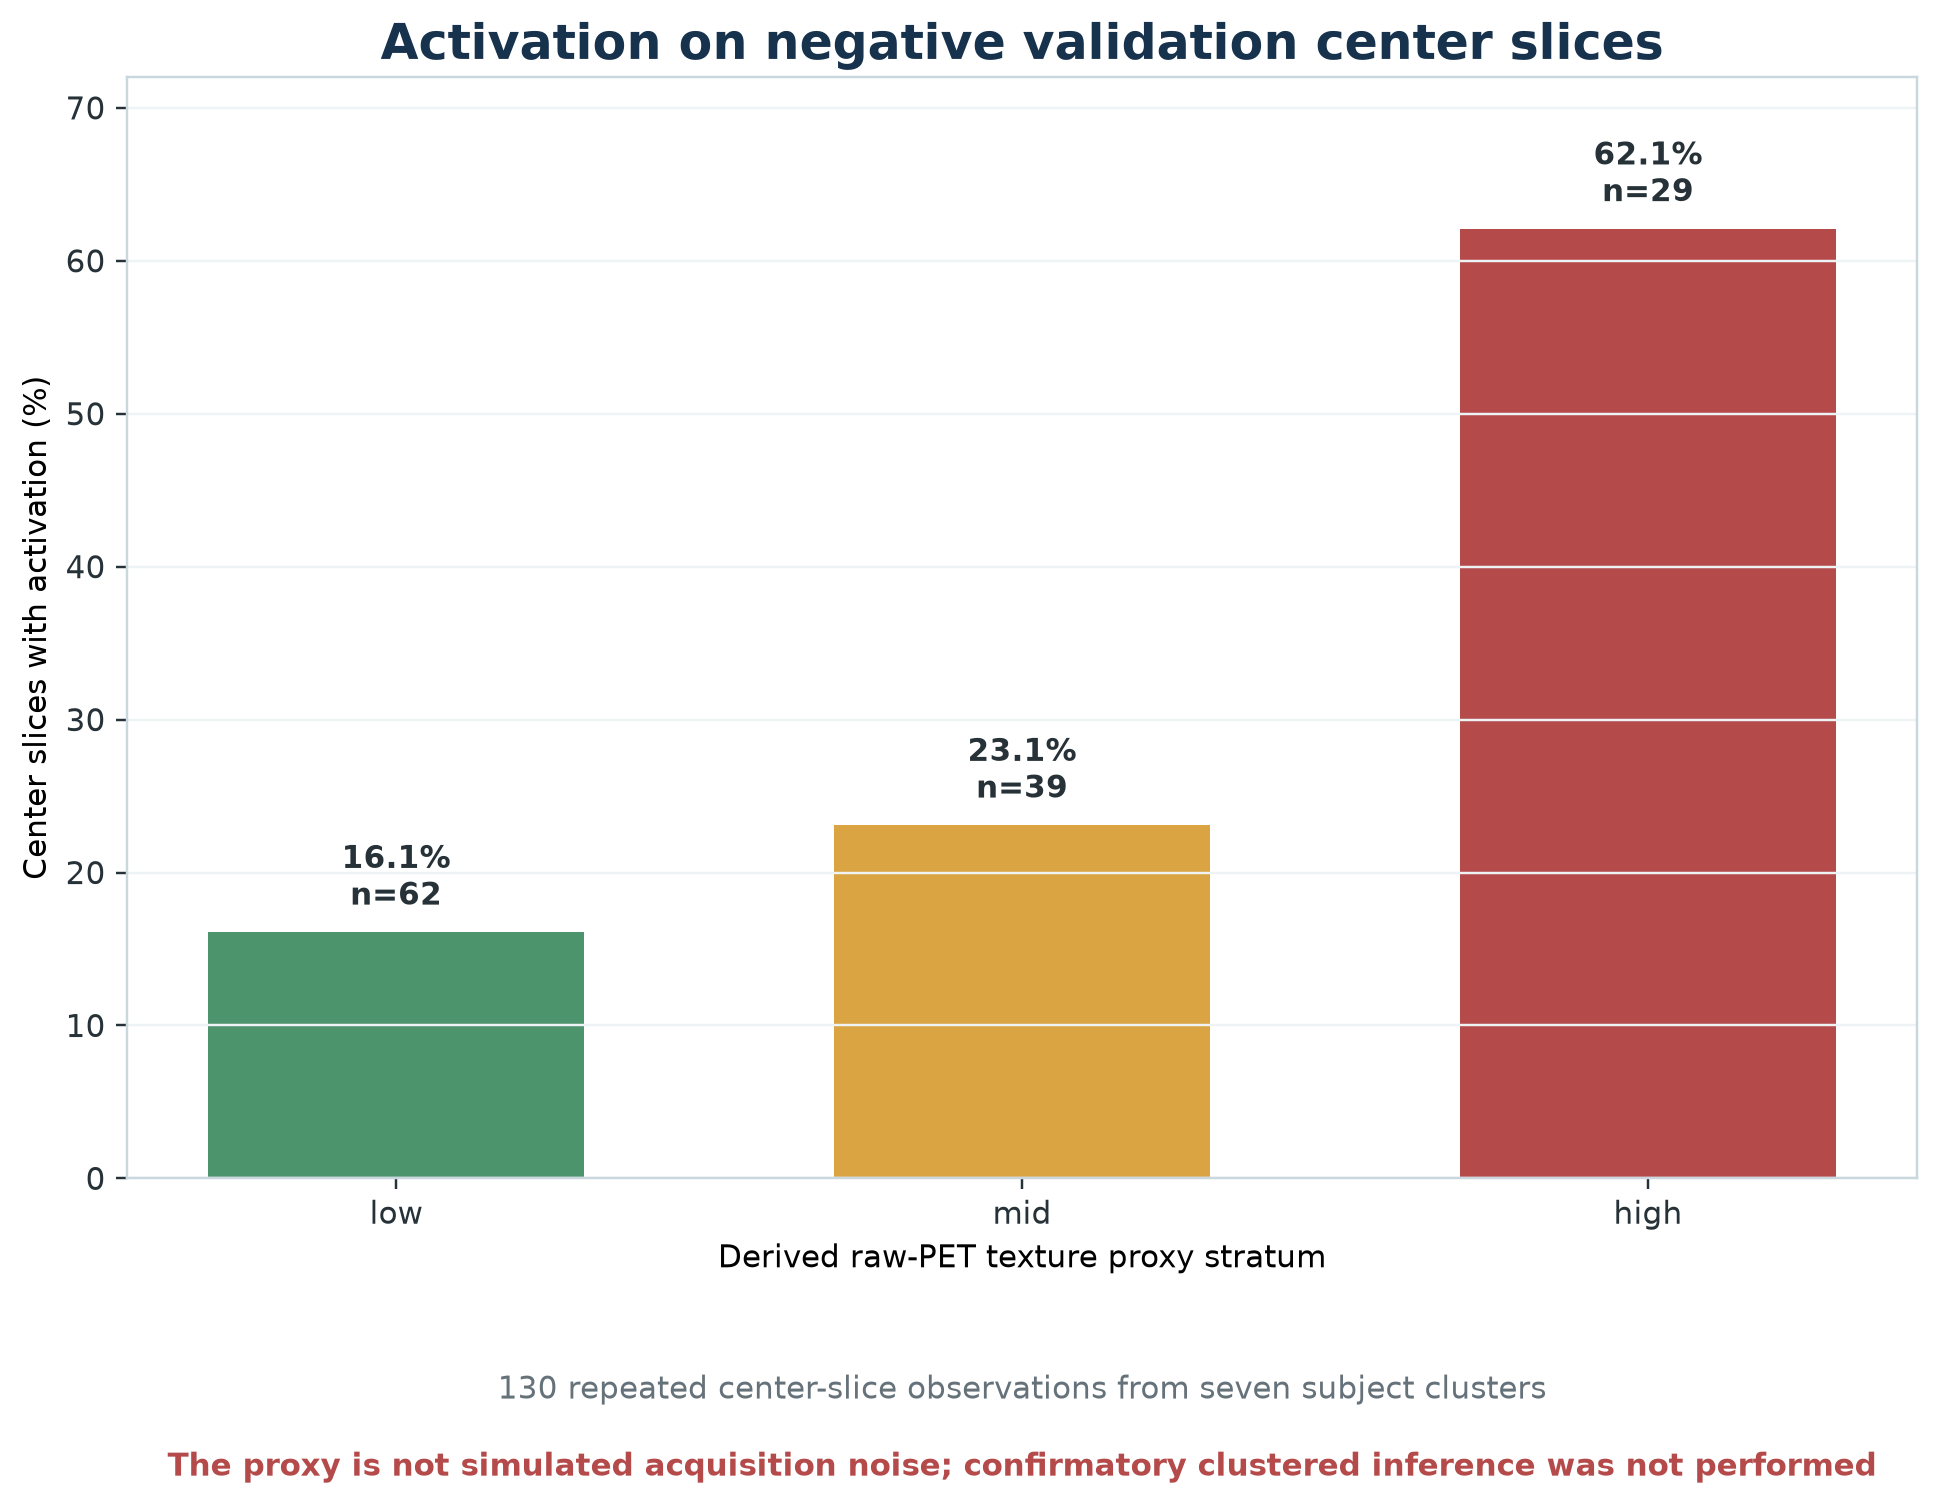
\includegraphics[width=0.88\textwidth]{figures/07_activation_by_noise_proxy.png}
\caption{Activation by derived raw-PET texture proxy. Population: 130 negative validation center slices from seven subject clusters. Unit: percent of center slices with any activation. The strata have 62, 39, and 29 repeated observations. The x-axis is not simulated acquisition noise, and the plot does not support clinical false-positive language or confirmatory inference.}
\label{fig:texture}
\end{figure}

\subsection{What the atlas does and does not show}

The atlas locates weak conditions in the current image-domain experiment. Small radius and high blur are associated with lower mean overlap in this cache. Uptake is not monotonic. High background texture is associated with more negative-slice activation descriptively. These observations can guide a final error taxonomy and prespecified stress set.

The atlas does not establish a biological detection threshold, a scanner limit, an acquisition recommendation, or generalization to vascular disease. It also does not include a valid CT-input registration stress because the stored shift was not applied.

\section{Deterministic quantification}

\subsection{Standalone 3D quantifier}

The standalone quantification module is designed to receive raw SUVbw, a target mask, grid geometry, a physical reflection transform, and an optional world-space centerline direction. It computes:

\begin{itemize}
  \item target SUVmax and SUVmean from raw native SUVbw;
  \item mask volume in mL using voxel count times $|\det(A_{3\times3})|/1000$;
  \item longitudinal extent as the maximum minus minimum projection of occupied physical points along the supplied fixed direction, or along the mask principal-component axis when no direction is supplied;
  \item contralateral SUV values from a reflected physical region;
  \item asymmetry and target-to-contralateral ratios after denominator validation;
  \item QC flags for empty masks, boundary contact, fragmentation, and small targets, with structured null reasons for invalid reflected regions.
\end{itemize}

Invalid measurements are represented as structured nulls with typed reasons. A zero value is retained only when zero is a valid measurement. Keeping those cases distinct prevents an empty predicted mask from being reported as a measured zero.

The implemented extent is a straight-axis physical projection. It does not follow a curved centerline. Curve-following arc-length measurement is unimplemented.

\subsection{Missing aggregate quantification evidence}

No report-ready aggregate evaluation of SUV error, volume error, extent error, contralateral ratio error, or laterality accuracy was available for the selected B2 model. The existence of formulas and unit tests does not establish measurement accuracy on the validation cache. A final evaluation should compare predicted-mask measurements with synthetic ground-truth measurements and preserve every invalid case in the denominator.

\subsection{Product integration gap}

The product demonstration does not yet invoke the complete 3D engine for its learned backend. It processes one 2D center slice. The adapter computes target SUVmax and SUVmean from the available raw SUVbw slice only when the predicted mask is nonempty and its target values are finite. It does not convert clipped contralateral channels or pixel counts into physical measurements. Instead, it returns structured nulls with typed reasons when the mask is empty, raw contralateral SUV is unavailable, in-plane spacing is missing, longitudinal extent cannot be derived, or target SUV is nonfinite. Laterality remains an approximation based on the array midpoint. Structured nulls prevent unavailable quantities from appearing as numeric measurements, but they do not complete 3D physical quantification.

Closing this gap requires the product to pass a stitched native PET-grid mask, the original raw SUV volume, the frozen reflection transform, and, when available, the frozen world-space centerline direction into the standalone quantifier. It must then copy the resulting structured measurements without rewriting them.

\section{End-to-end product pipeline}

\subsection{Implemented product flow}

The product code exposes a single local orchestration path with a serializable tool registry. The high-level flow is: load a case, select a detection backend, assemble deterministic metrics, optionally retrieve evidence, generate a structured research report, and verify that report against the source measurements and claim rules. A Streamlit interface presents the research artifacts. A local Model Context Protocol server exposes the same tool layer and restricts artifact access to a configured output root.

The report path defaults to a deterministic template. Optional language generation is restricted to interpretation and limitations prose. Numeric fields are copied from structured measurements. If the optional generation stack is unavailable, the product falls back to the template. A deterministic verifier compares every numeric field, checks laterality, requires synthetic status, and screens specified prohibited claims.

\subsection{Detection backends}

The default \texttt{reference} backend creates a synthetic demonstration case, returns the known synthetic mask, and uses a fixed \scoreterm\ of 0.91. It is a deterministic integration fixture, not a detector benchmark. It proves that the application can route artifacts through the tools, report schema, verifier, and UI.

Its contralateral axis flip, mask-count divided by 1,000 nominal volume, and occupied-axial-plane count multiplied by 2 mm nominal extent are deterministic integration-fixture conventions. They are not physical-coordinate 3D scientific measurements and are not outputs of the standalone quantifier.

The opt-in learned backend loads the banked B2 checkpoint and processes one selected cached validation center slice. It fails on a missing checkpoint rather than silently returning the reference output. This path connects the model and product code, but it remains a single-slice research demonstrator. The selected slice must never stand in for the complete validation distribution.

\subsection{Evidence retrieval status}

The product includes optional two-stage local retrieval with dense embeddings followed by reranking. The earlier local index is excluded from this publication because its source set was broader than the approved public corpus. The default corpus builder now reads only \path{knowledge/research_corpus.json}; documentation folders are included only when an audited path is supplied explicitly. This is a safer default, but the sanitized index has not yet been rebuilt or reevaluated. Retrieval scores from the excluded snapshot are intentionally omitted.

A valid retrieval evaluation must begin after the public corpus is frozen. It should record corpus hashes, query construction, relevance labels, top-k recall, reranked ranking metrics, and failure examples. Report generation should retain evidence identifiers and fail closed when a claim has no supporting passage.

\begin{figure}[H]
\centering
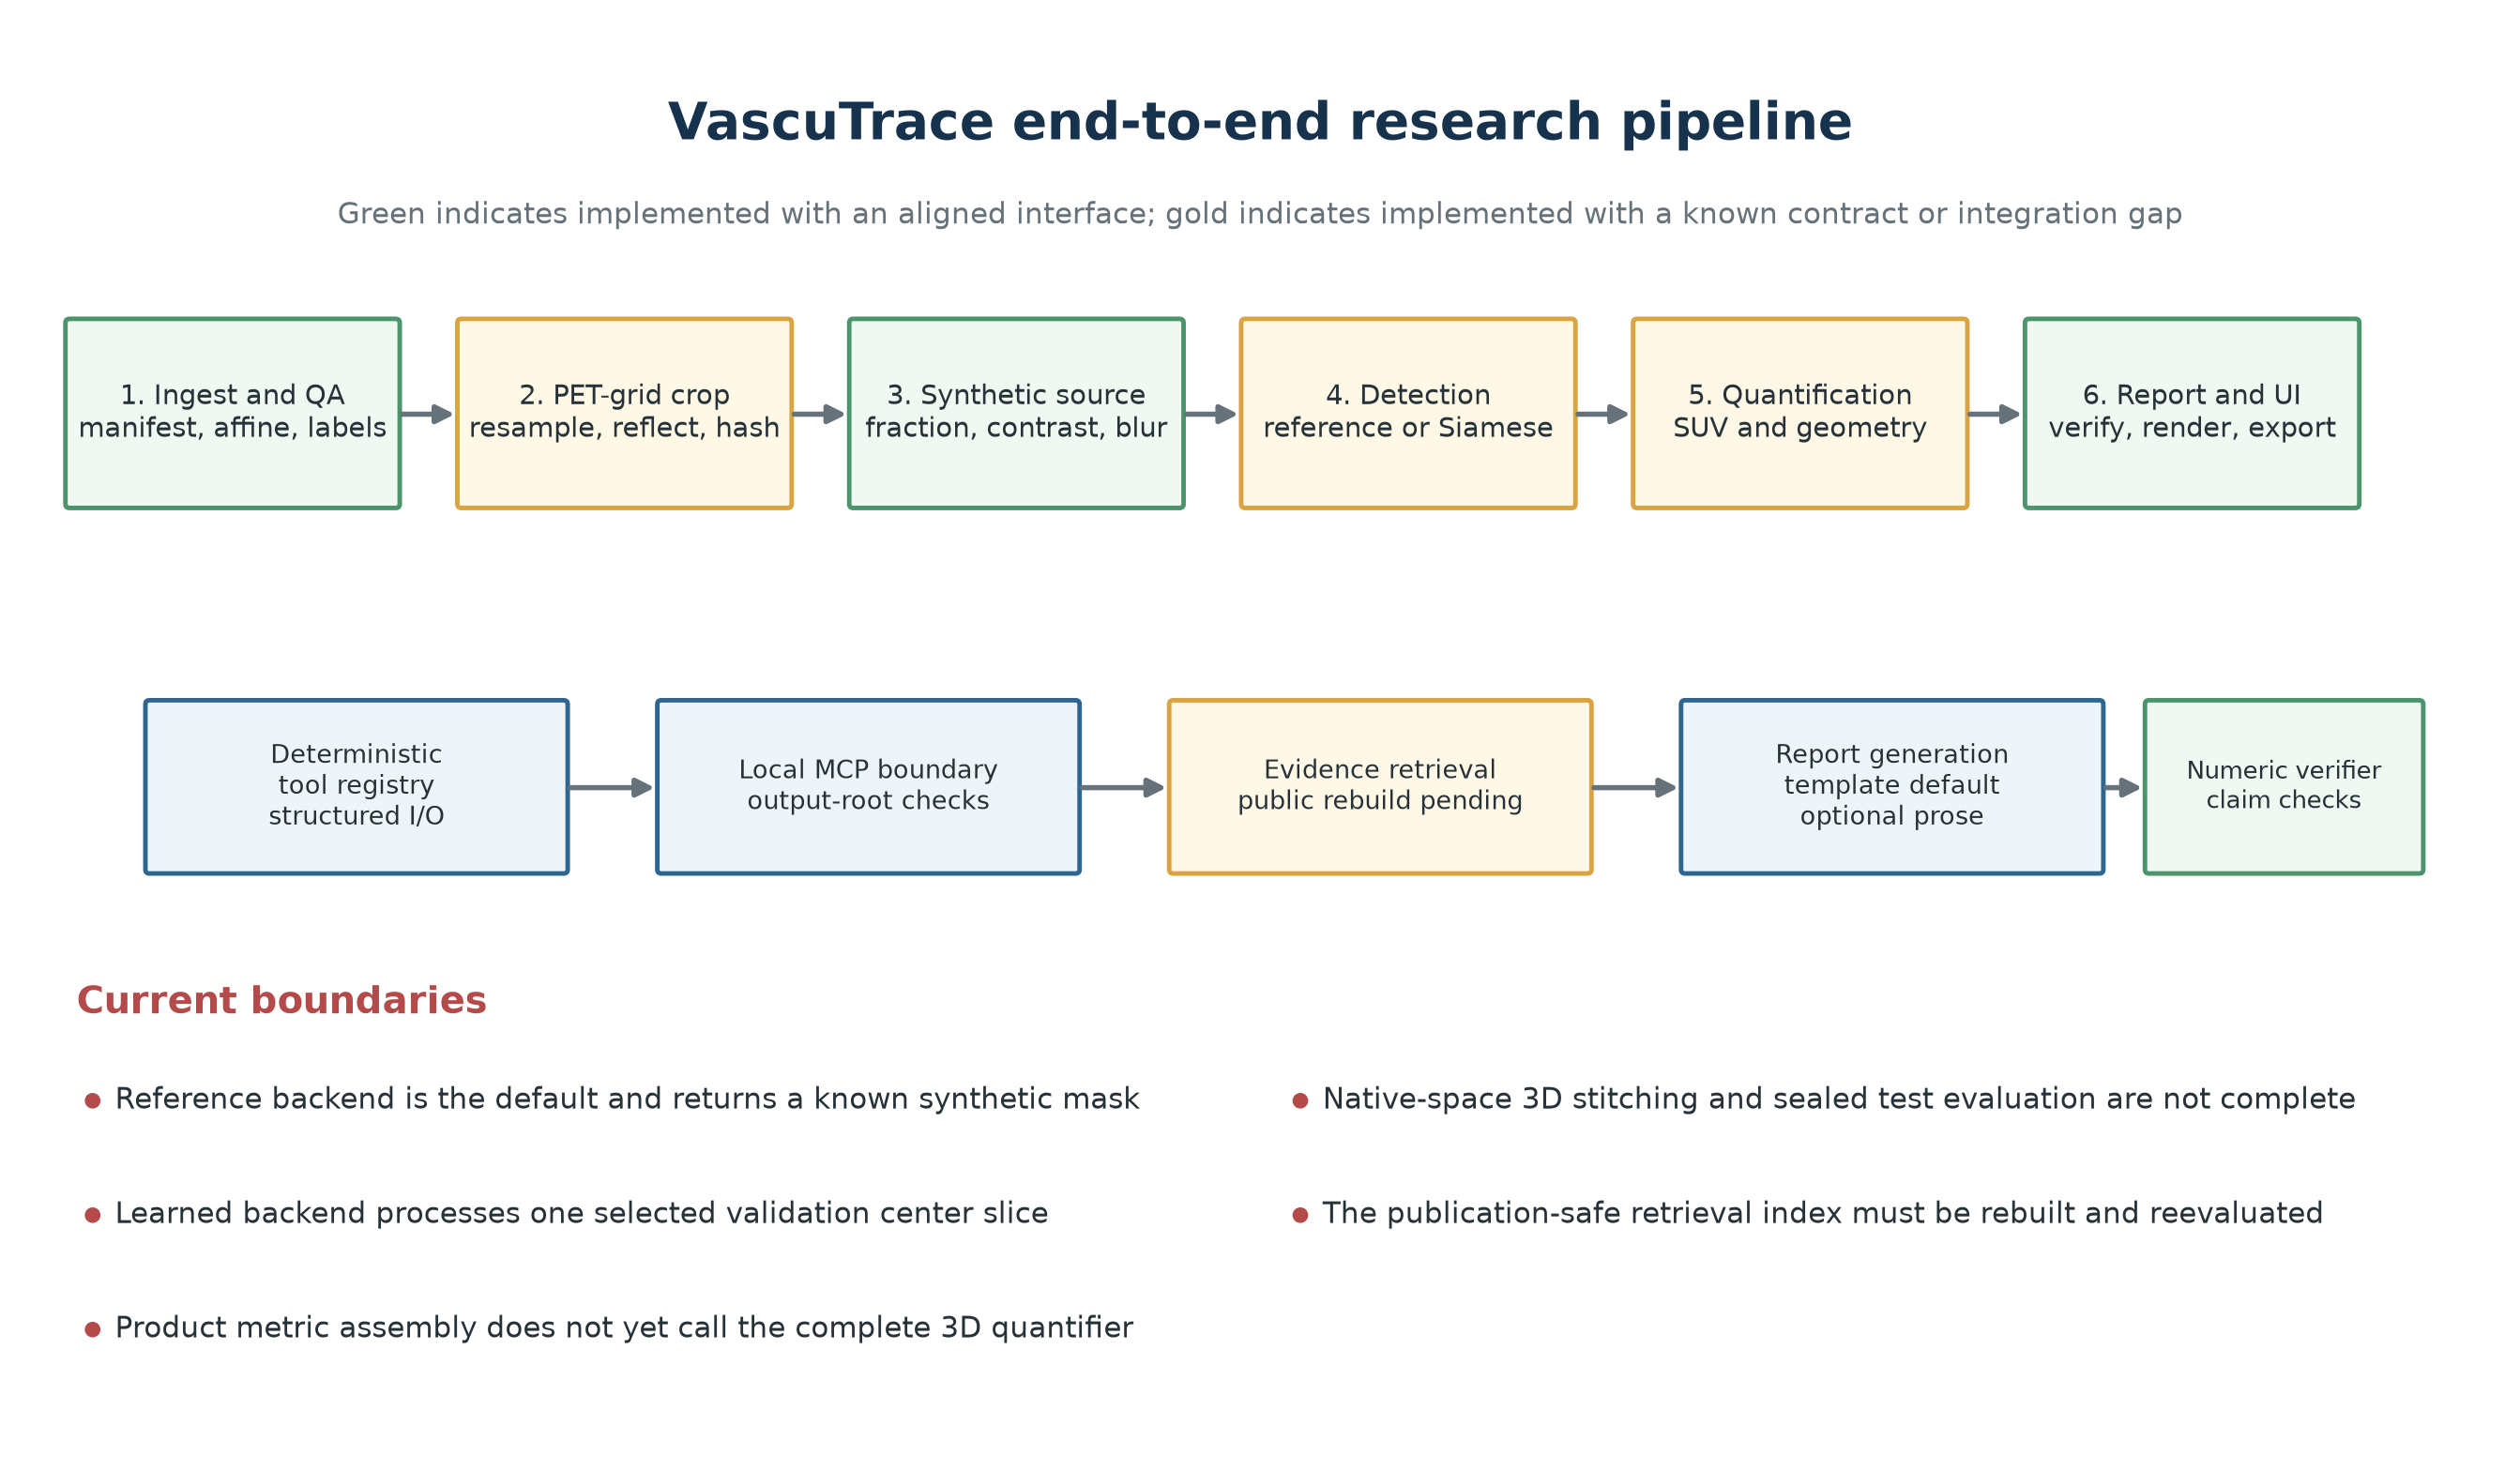
\includegraphics[width=0.99\textwidth]{figures/08_end_to_end_pipeline.png}
\caption{End-to-end research pipeline and current boundaries. Population: implemented modules and intended interfaces. Unit: pipeline stage. The figure is a generated schematic, not a run receipt. Green stages have an aligned public interface; gold stages contain a known contract or integration gap. The default reference backend is a fixture, the learned backend is one validation center slice, complete 3D quantification is not integrated, and the public retrieval index awaits rebuilding.}
\label{fig:pipeline}
\end{figure}

\subsection{Stage-by-stage status}

\begin{longtable}{B{0.14\textwidth} L{0.24\textwidth} L{0.24\textwidth} L{0.21\textwidth}}
\caption{Pipeline implementation status. The unit is a software or evaluation stage. Evidence comes from current code and historical aggregate receipts; no row implies clinical readiness.}\label{tab:pipeline-status}\\
\toprule
Stage & Current evidence & Main gap & Completion test \\
\midrule
\endfirsthead
\toprule
Stage & Current evidence & Main gap & Completion test \\
\midrule
\endhead
Ingest and QA & Strict inventory, grid checks, label presence, provenance fields, and typed errors & Archive-era label semantics remain provisional & Pin label map and run complete cohort eligibility with visual pelvis QA \\
Geometry and crop & PET reference grid, resampling helpers, fixed crop, reflection metadata, hash checks & Legacy reflection method differs from intended contract & Regenerate versioned crops and pass off-center, oblique, side-swap, and involution fixtures \\
Simulation & Fractional source, contrast, heterogeneity, blur, sham, and provenance & No acquisition-noise model; CT shift not applied in standard cache & Run factor-isolation tests and CT-input-only registration stress \\
Threshold baseline & Transparent score maps, components, threshold sweep, and infeasible status & Negative-scan F2 and physical-volume contract incomplete & Rebuild under one promotion-compliant validation protocol \\
Learned model & Callable B2 model, training configuration, checkpoint metadata, center-slice evaluation & No native 3D stitching or sealed test & Freeze model and operating point, then run one subject-level test evaluation \\
3D metrics & Standalone raw-SUV 3D formulas; 2D adapter uses structured nulls for unavailable physical values & Complete 3D quantifier is not integrated into the product & Route native masks and geometry into the standalone quantifier and measure errors \\
Retrieval and report & Template default, approved JSON corpus default, optional explicit document paths, numeric verifier & Public index not rebuilt; verifier scope remains finite & Rebuild corpus, evaluate retrieval, and run adversarial report-fidelity tests \\
UI and export & Research demonstrator and artifact views & Single-slice learned demonstration & Display complete scan status, null reasons, provenance, and aggregate uncertainty \\
\bottomrule
\end{longtable}

\section{Executed product and collaboration evidence}

\subsection{Reproducible generated-only execution}

The report evidence builder executes the default product path in a temporary directory. Detection uses the \texttt{reference} backend. Reporting uses \texttt{template}, and evidence uses \texttt{keyword}. The builder runs the complete synthetic-case command, materializes the five display views used by the dashboard, verifies the structured report, and runs the six-case product evaluation. It removes temporary paths and runtime durations before writing \path{docs/report/evidence/product_demo_receipt.json}. The receipt and Figures~\ref{fig:generated-product-case}--\ref{fig:collaboration-evidence} are bound to evidence record \evidenceid{DEMO-001}. The execution makes no dataset read, model-weight read, network request, or API call.

The executed fixture was \texttt{synthetic\_iliac\_seed\_182}. Its metadata stores the label right, radius 5.0 mm, axial length 16.0 mm, uptake multiplier 1.6, and seed 182. These values are nominal fixture labels, not generation controls or measurements from a person. The current deterministic array generator does not use the stored seed, radius, or length and does not apply the stored uptake multiplier. It uses a fixed binary source mask and adds a fixed 0.76 SUV increment inside that mask. Figure~\ref{fig:generated-product-case} presents the actual PNG output of the product view generator rather than a conceptual diagram.

\begin{figure}[H]
\centering
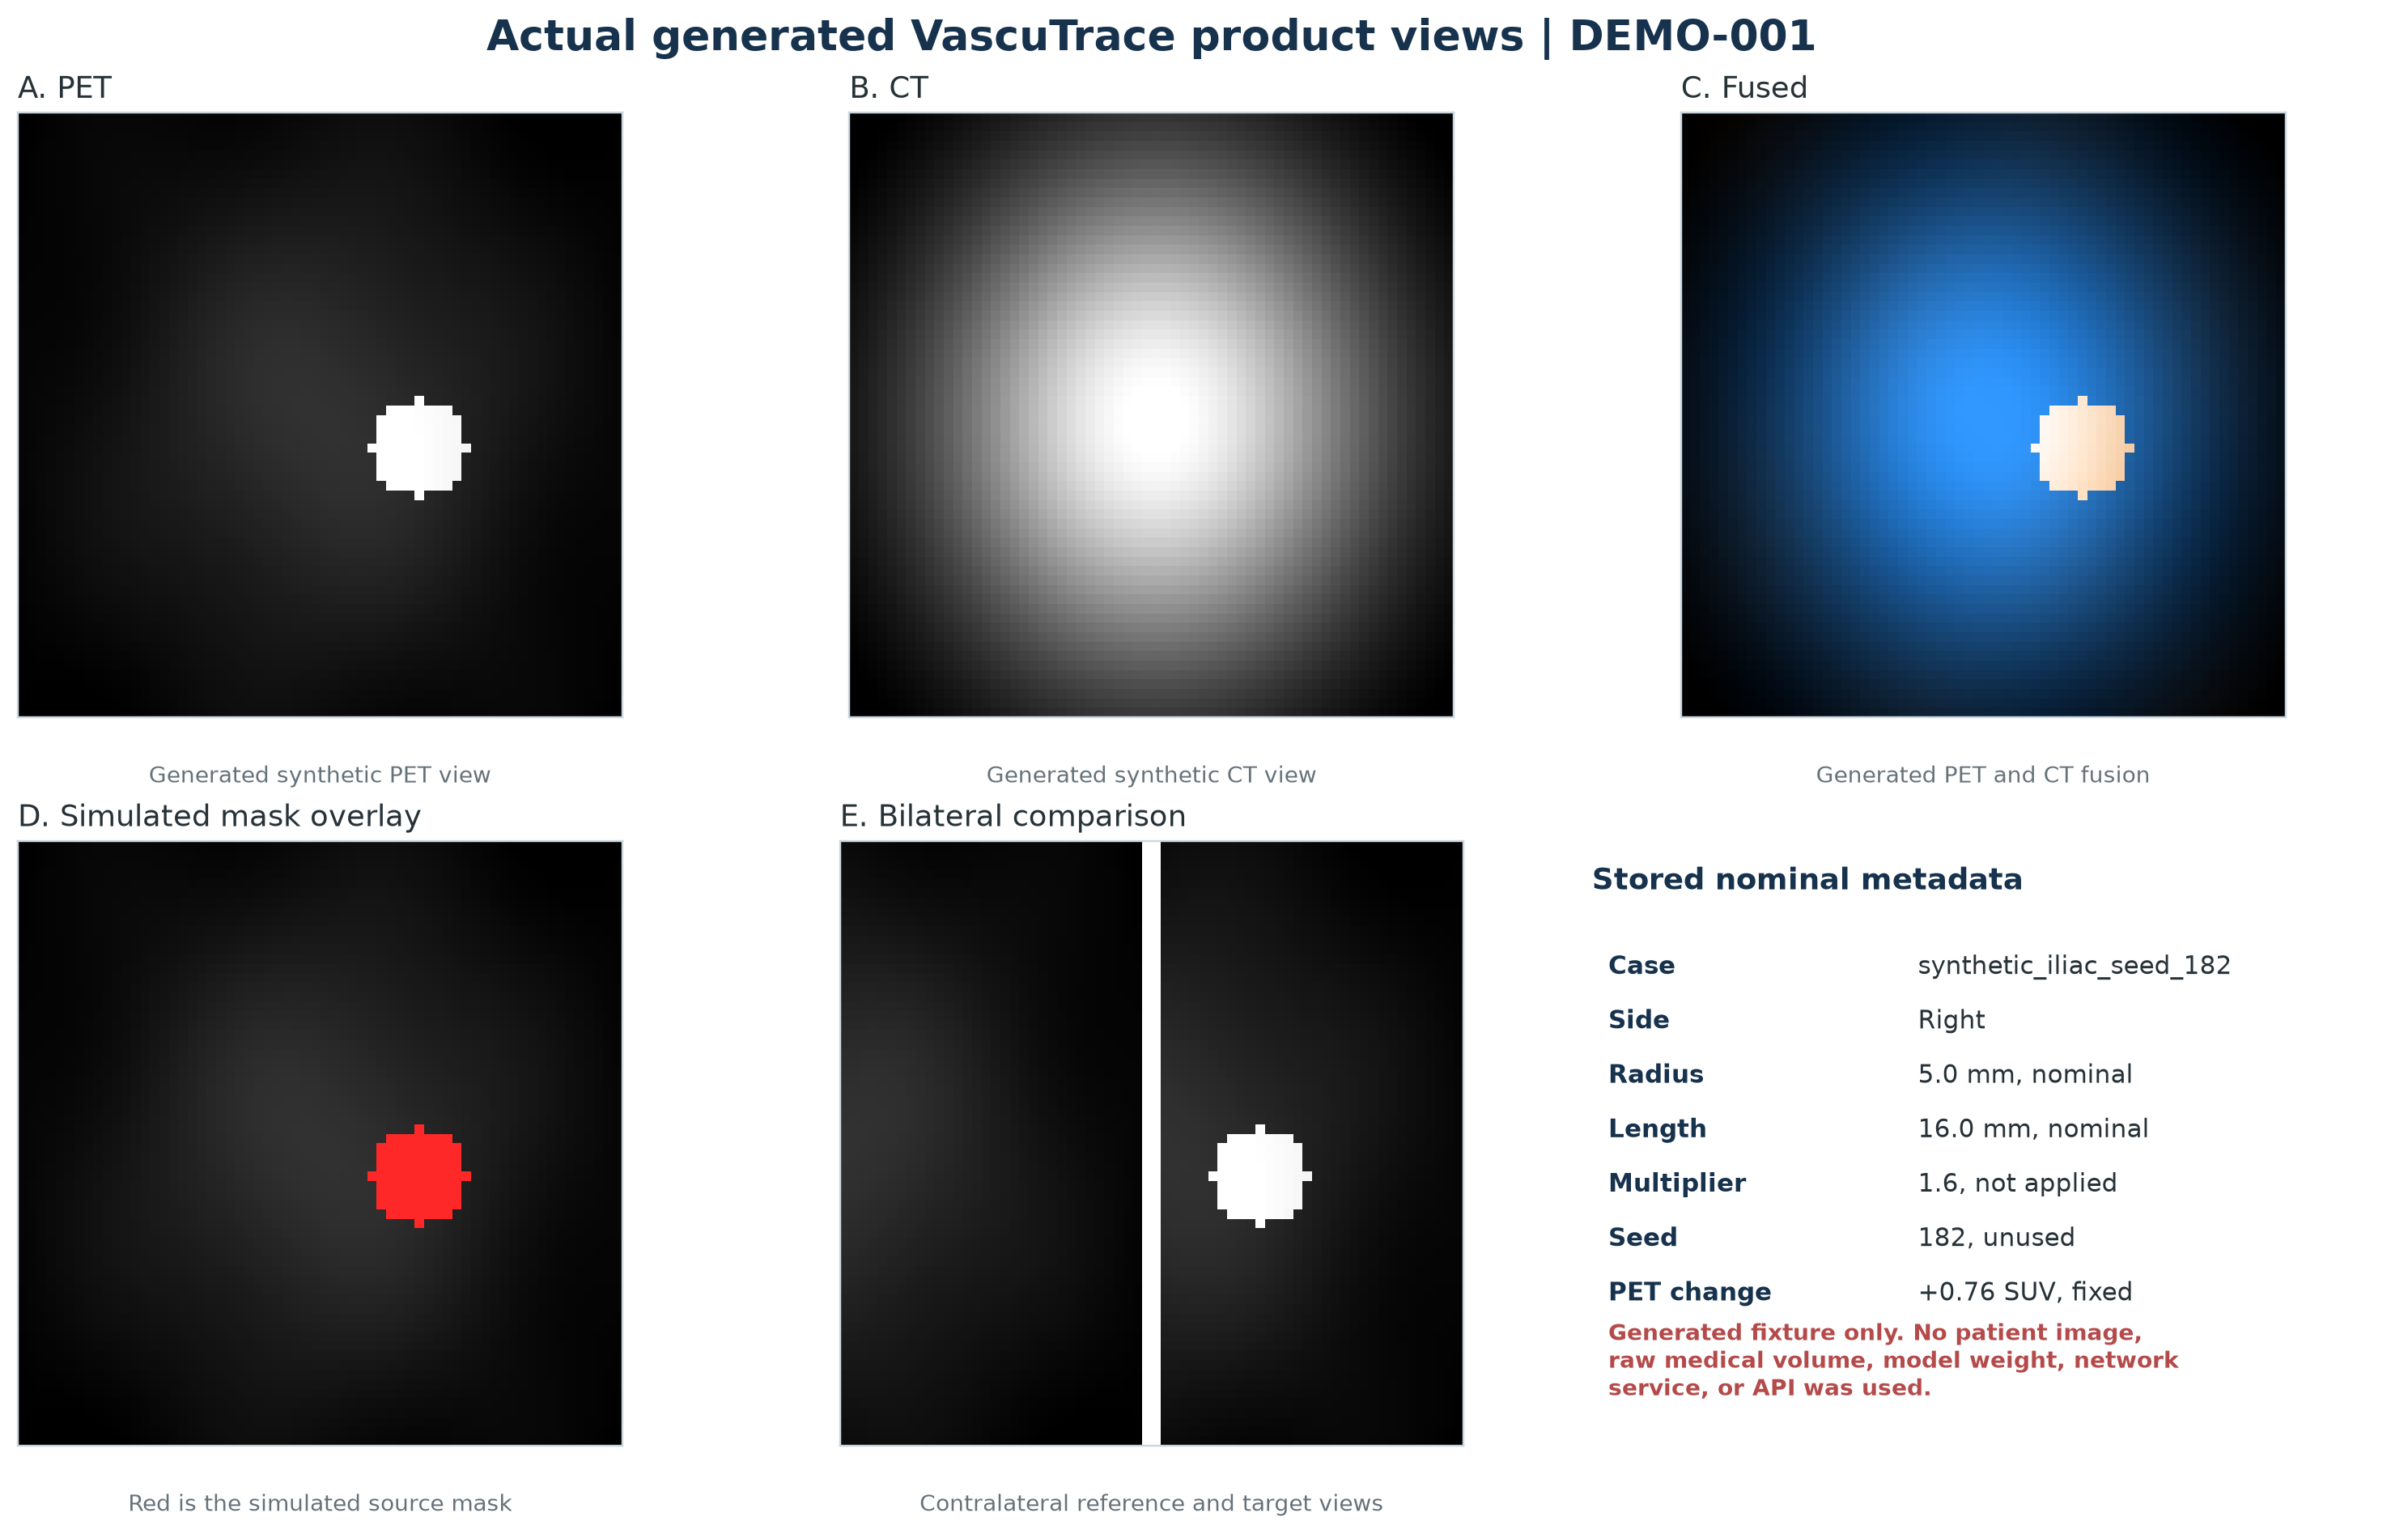
\includegraphics[width=0.99\textwidth]{figures/09_generated_product_case.png}
\caption{Actual generated VascuTrace product views. Evidence ID: \evidenceid{DEMO-001}. Population: one deterministic synthetic integration fixture, not a patient or a patient-derived image. The source arrays have shape $16 \times 64 \times 64$; the displayed middle-slice PET, CT, fusion, and overlay views are $64 \times 64$ pixels, and the bilateral view is $64 \times 66$ pixels including its separator. The bright right-sided region and red overlay show the simulated source. Radius, length, multiplier, and seed are stored nominal metadata; the generator uses a fixed mask and a fixed 0.76 SUV increment. The panels validate image production and UI inputs only. They do not establish anatomical realism, physical geometry, detector performance, or clinical behavior.}
\label{fig:generated-product-case}
\end{figure}

\subsection{Deterministic values and report verification}

Table~\ref{tab:executed-fixture} copies the stored JSON values from the generated receipt. The report verifier accepted the structured report with zero issues, and the report measurements were identical to the deterministic metric object. The fixed reference backend reported right laterality and an uncalibrated \scoreterm{} of 0.91. Its known target mask is intentionally used to exercise product wiring. This execution is not a model benchmark.

\begin{table}[H]
\centering
\caption{Executed default-path values copied from the structured receipt. Population: one generated synthetic integration fixture. Unit: SUV, mL, mm, or unitless as shown. Limitation: these are integration-fixture conventions, not physical-space 3D scientific measurements.}
\label{tab:executed-fixture}
\begin{tabularx}{\textwidth}{B{0.30\textwidth} Y L{0.18\textwidth}}
\toprule
Field & Stored JSON value & Unit or status \\
\midrule
Target SUVmax & 1.6534085273742676 & SUV \\
Target SUVmean & 1.6277599334716797 & SUV \\
Contralateral SUVmax & 0.8860967755317688 & SUV \\
Contralateral SUVmean & 0.8562601208686829 & SUV \\
Asymmetry index & 0.9010110290086896 & Unitless \\
Nominal metabolic volume & 0.648 & mL convention \\
Nominal longitudinal extent & 16.0 & mm convention \\
Report verification & Accepted; zero issues & Deterministic check \\
\bottomrule
\end{tabularx}
\end{table}

The two geometric-looking values require special care. The reference path calculates nominal volume as positive-mask voxel count divided by 1,000 and nominal extent as the number of occupied axial planes multiplied by 2 mm. The contralateral region is an array-axis reflection. Those rules are stable integration conventions, but they do not use the full physical-coordinate 3D quantifier, the subject-specific reflection plane, or curve-following centerline distance. The completed straight-axis quantifier itself reports projected extent, not curved centerline arc length. The new evidence therefore preserves both the projected-extent correction and the fixture-metric validity boundary.

\subsection{Observed runtime trace and product checks}

The runtime trace contained exactly the five tools shown in Figure~\ref{fig:verified-product-output}, in that order. This trace shows that code-owned measurements are produced before report generation and are checked afterward. It is a product execution trace, not a development-agent transcript or a hidden reasoning record.

The product evaluation passed all six checks and failed none. Table~\ref{tab:product-checks} states what each check established in this run.

\begin{table}[H]
\centering
\caption{Fresh default-path product evaluation. Population: six deterministic software checks over generated fixtures. Unit: check. Passing these checks establishes the listed integration safeguards only.}
\label{tab:product-checks}
\begin{tabularx}{\textwidth}{B{0.24\textwidth} L{0.16\textwidth} Y}
\toprule
Check & Outcome & Observable result \\
\midrule
Strict contracts & Pass & Model output and report satisfied strict versioned schemas. \\
Measurement preservation & Pass & Every report measurement exactly matched the deterministic source metric object. \\
Unsafe claim rejection & Pass & The verifier rejected an injected diagnostic claim. \\
Case-cache bypass & Pass & Repeated case-specific measurement queries bypassed the semantic cache. \\
Missing-artifact failure & Pass & A missing metrics artifact produced an explicit service failure. \\
Complete tool trace & Pass & Every required checkpoint tool appeared in the expected order. \\
\bottomrule
\end{tabularx}
\end{table}

\clearpage
\begin{figure}[p]
\centering
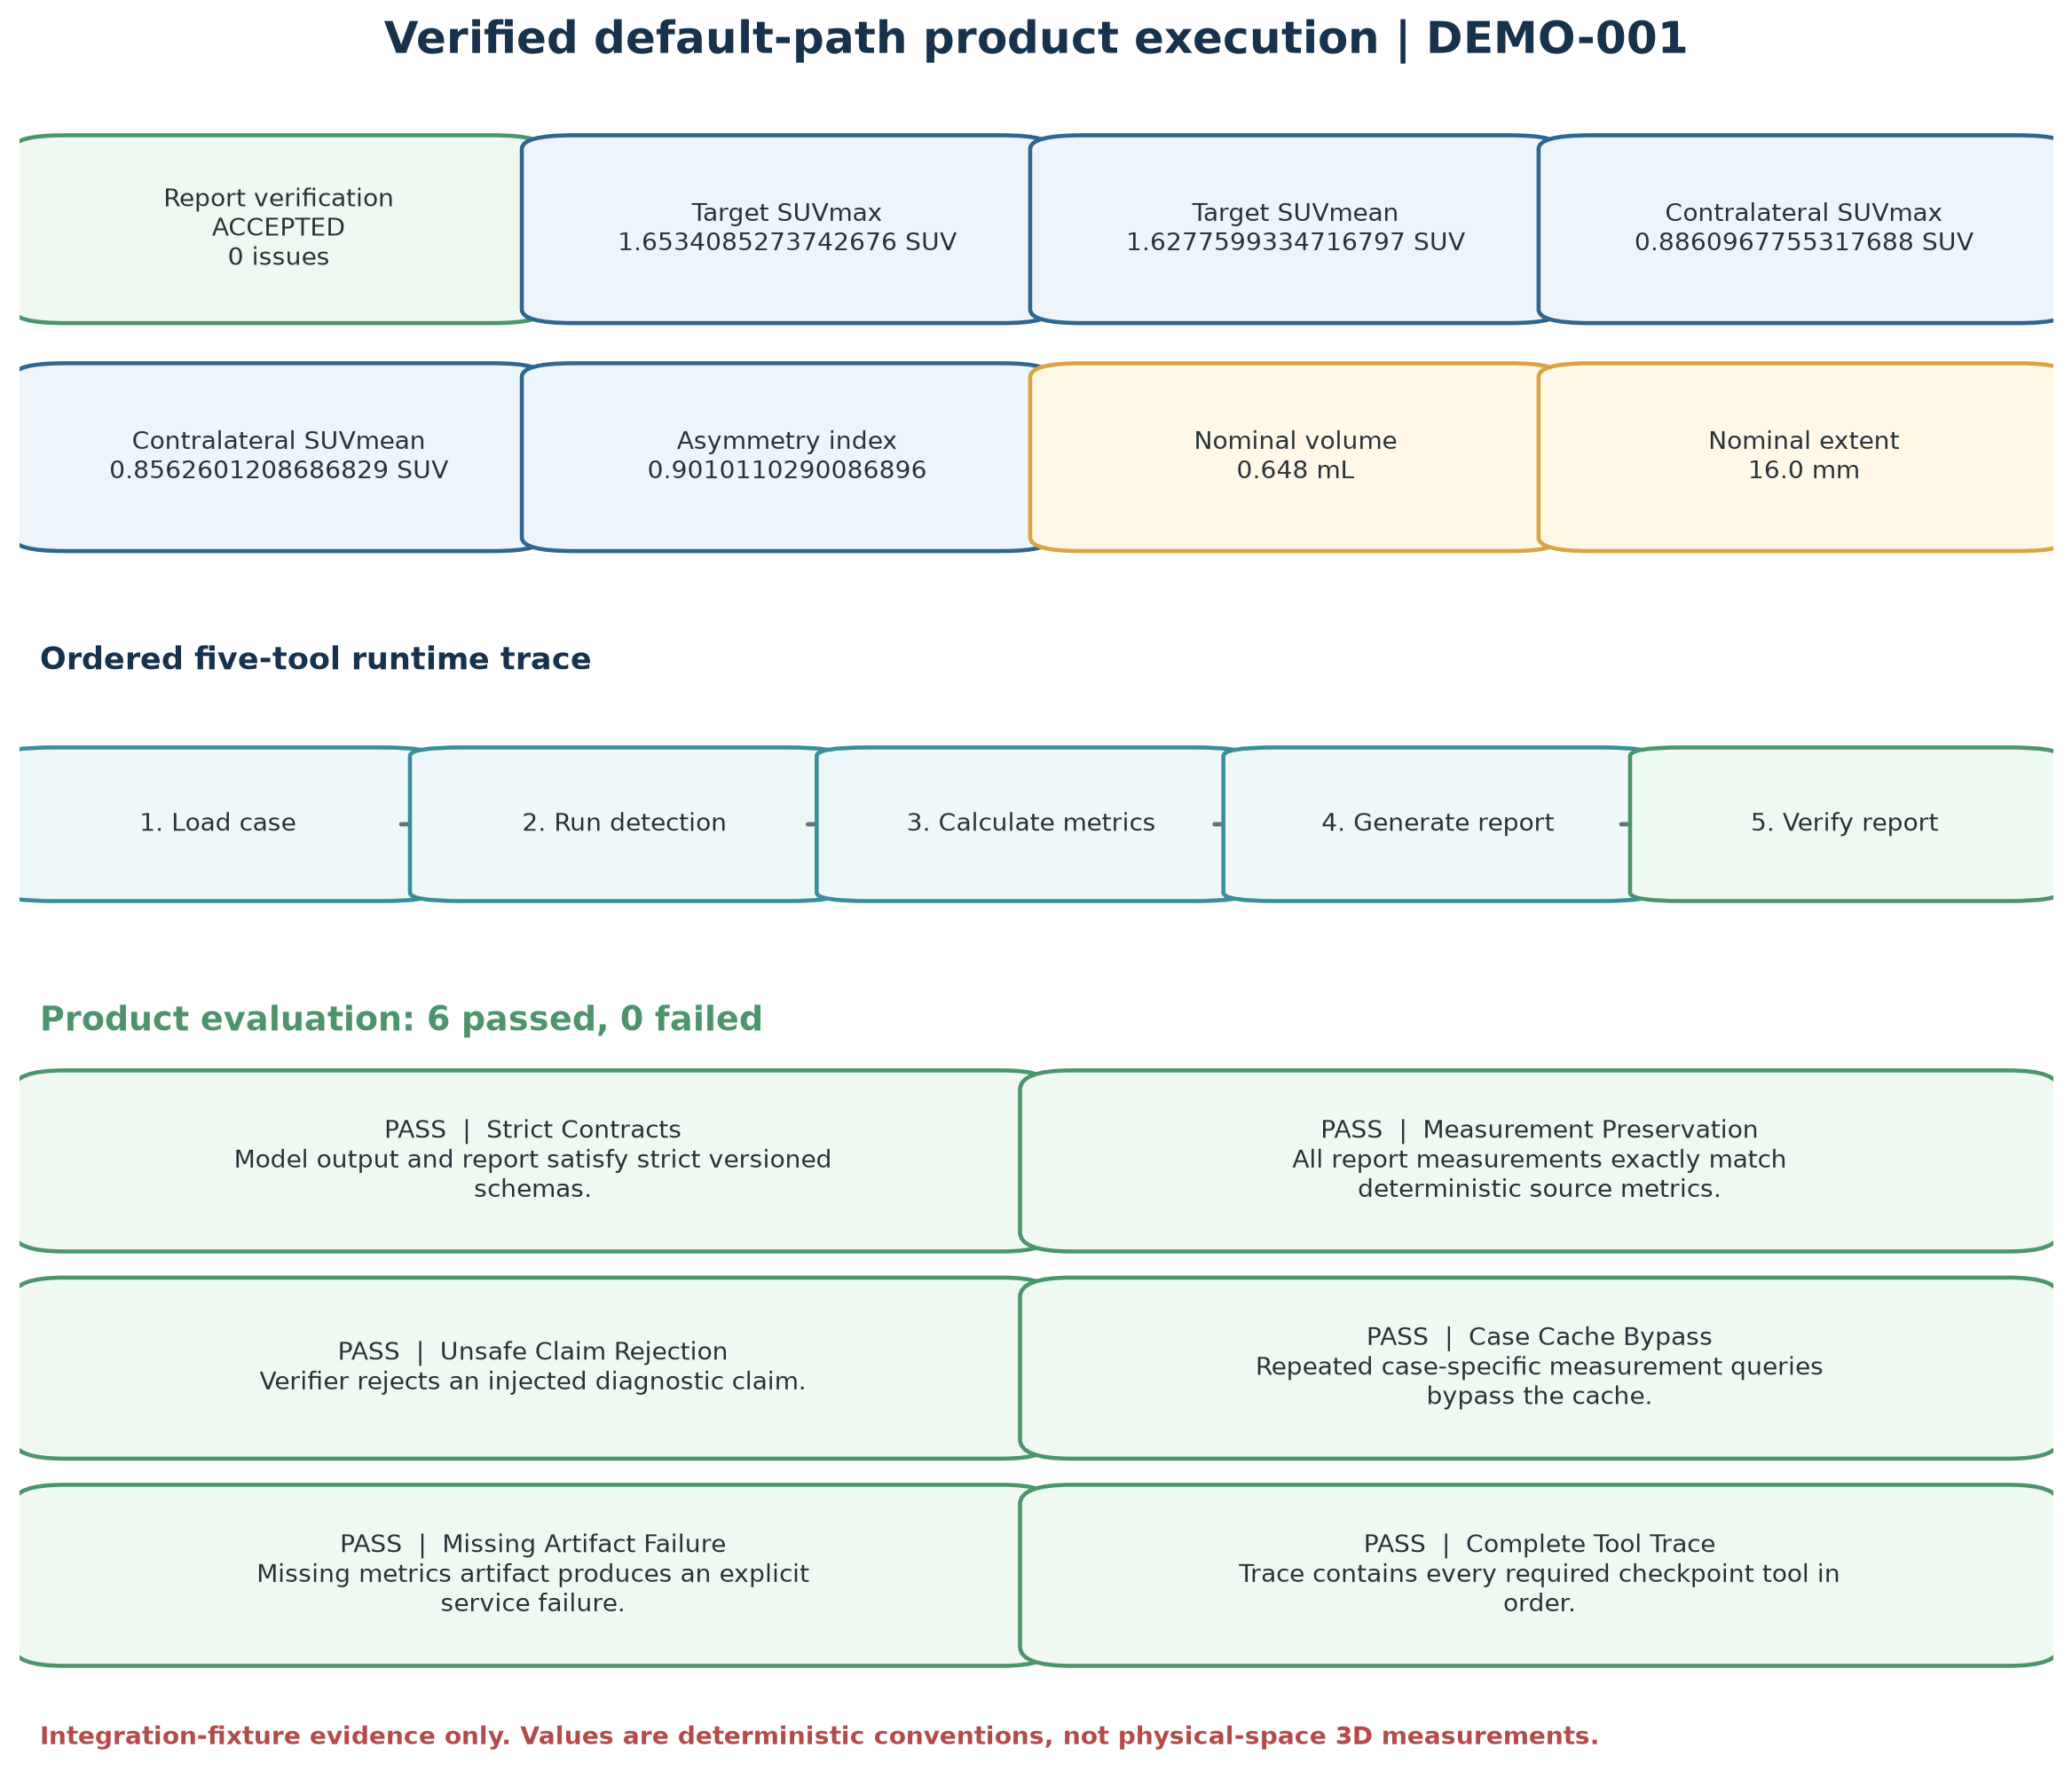
\includegraphics[width=0.94\textwidth]{figures/10_verified_product_output.png}
\caption{Verified default-path product execution rendered from the generated receipt. Evidence ID: \evidenceid{DEMO-001}. The top panel shows report acceptance and literal JSON values. The middle panel shows the ordered five-tool trace. The lower panel shows the six passed checks and their observed outcomes. The nominal volume and extent remain fixture conventions. No value in this figure is generated or rewritten by a language model.}
\label{fig:verified-product-output}
\end{figure}
\clearpage

\subsection{Development collaboration evidence}

Development collaboration is a separate evidence class from the VascuTrace product runtime. Codex with GPT-5.6 performed every non-coding workflow role. It owned planning and architecture, primary technical decisions, scientific review, report writing, delivery review, Git and release handling, and humanizer and editorial review. Codex also authored the plans and instructions used for code implementation. Claude implemented code only, following those instructions. The owner retained final product, engineering, scientific, publication, licensing, repository, category, video, and submission authority.

Figure~\ref{fig:collaboration-evidence} makes this ownership explicit. Scientific review, delivery review, and humanizer review were Codex with GPT-5.6 workstreams. They were not Claude coding responsibilities and were not performed by the shipped VascuTrace runtime agents. The publication plan, report source, collaboration record, and submission guide provide the public non-coding evidence. The dashboard, commands, runtime package, and tests provide public examples of the code implementation.

\clearpage
\begin{figure}[p]
\centering
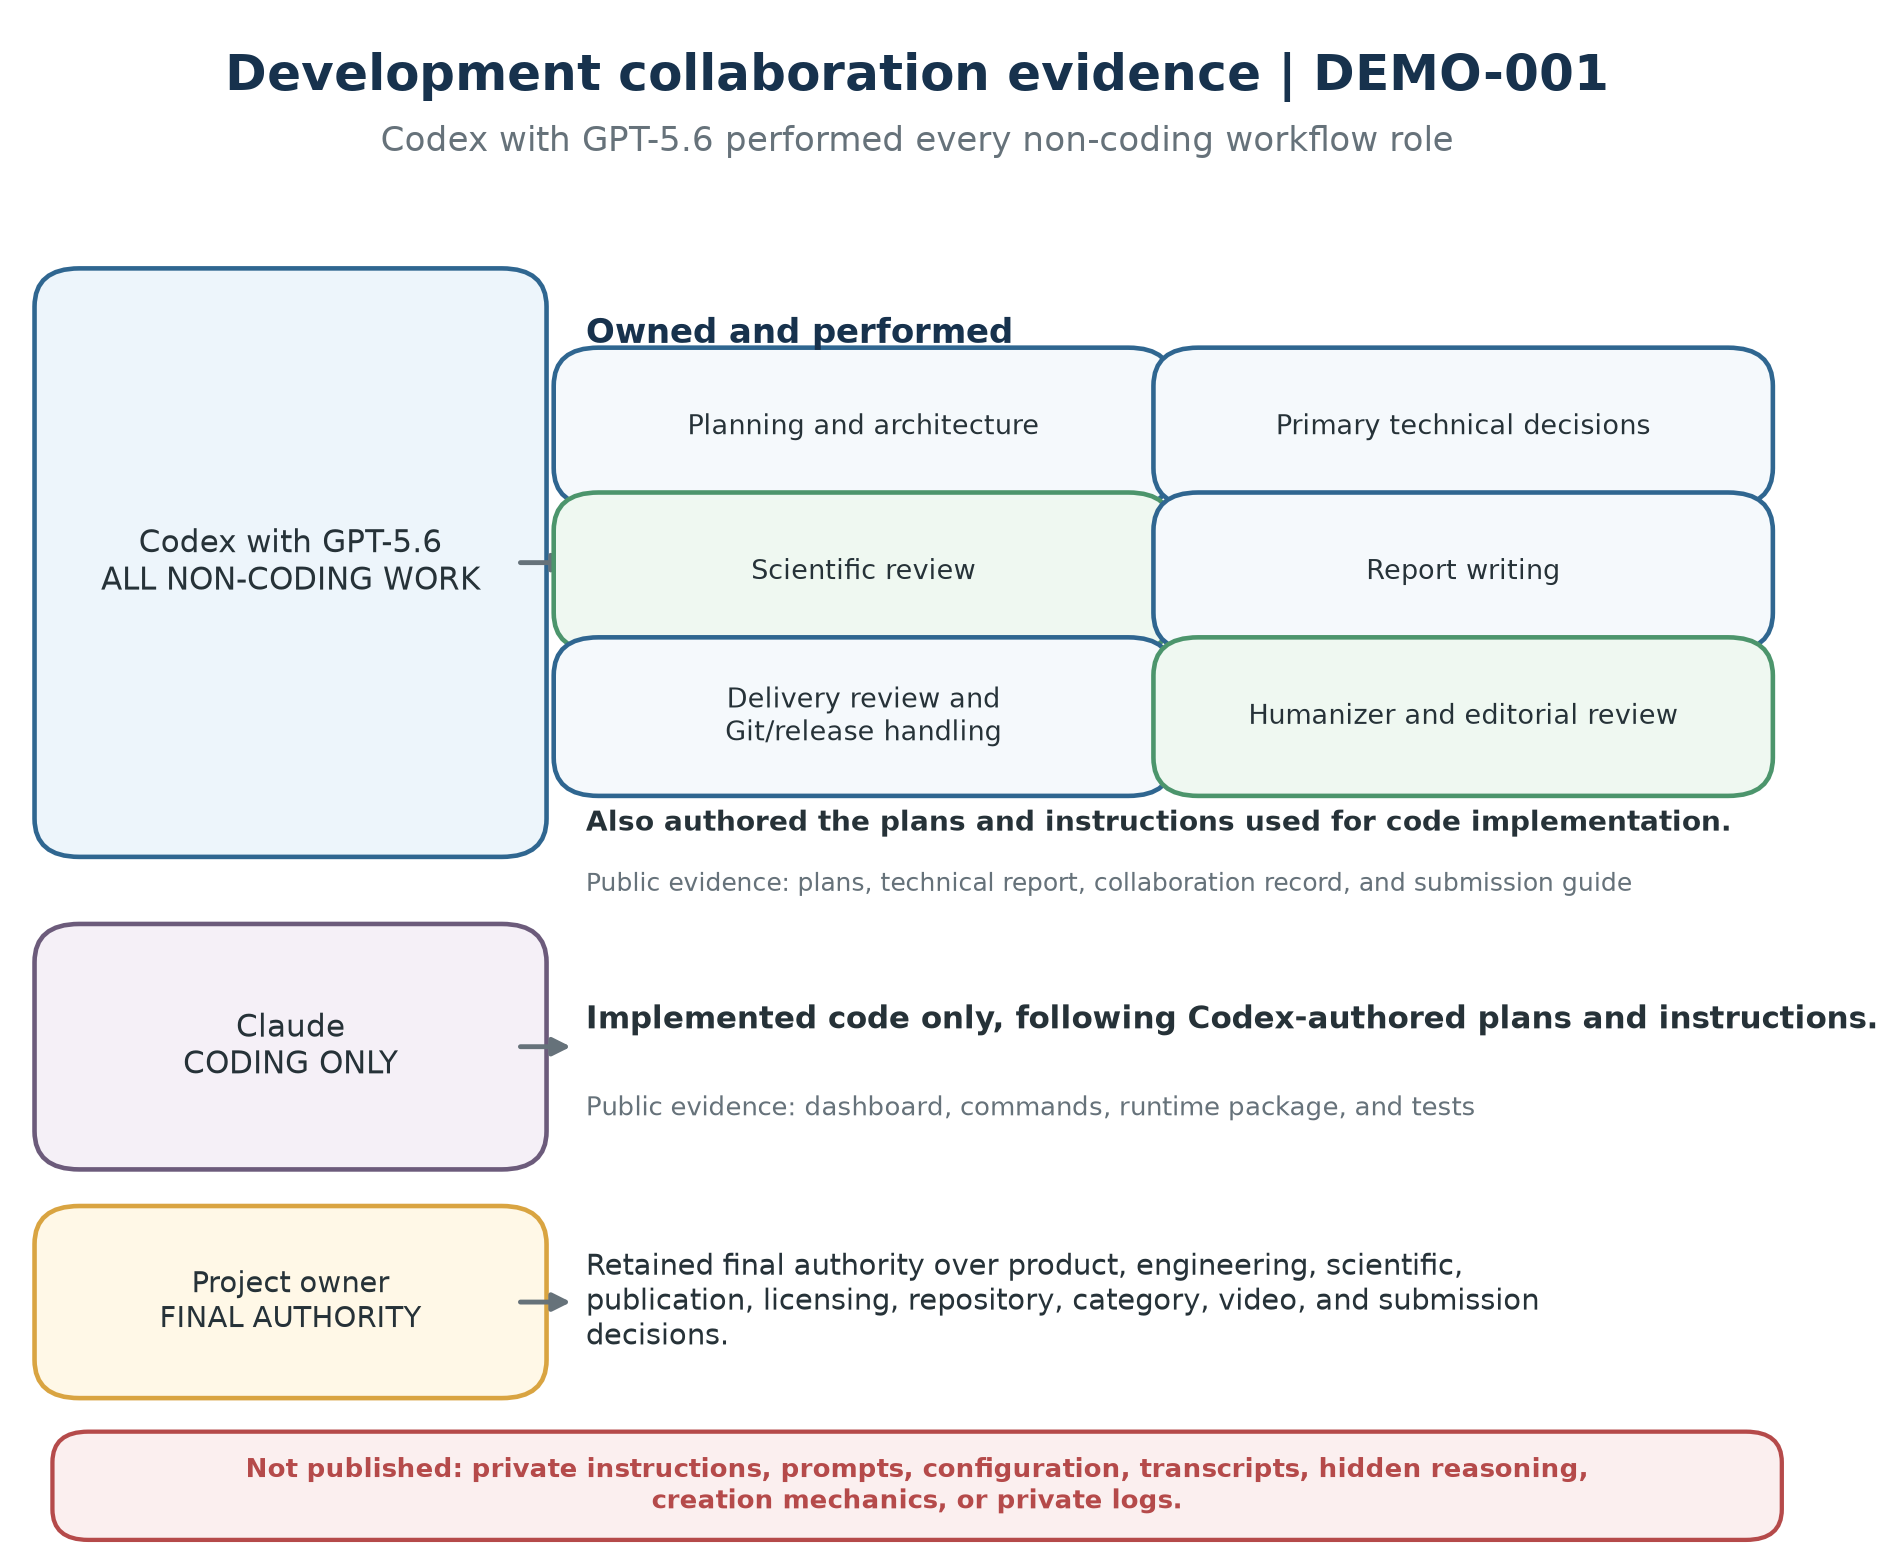
\includegraphics[width=0.94\textwidth]{figures/11_collaboration_evidence.png}
\caption[Development collaboration evidence.]{Development-collaboration ownership and public artifact links. Evidence ID: \evidenceid{DEMO-001}. Codex with GPT-5.6 performed every non-coding workflow role, including planning, primary technical decisions, scientific review, report writing, delivery review, Git and release handling, and humanizer and editorial review. It also authored the plans and instructions used for coding. Claude implemented code only. The owner retained final authority. These roles are separate from the VascuTrace product runtime. No private instruction, prompt, configuration, transcript, hidden reasoning, creation mechanism, subagent identifier, or raw log is reproduced.}
\label{fig:collaboration-evidence}
\end{figure}
\clearpage

\subsection{Codex root session evidence}

Evidence record \evidenceid{SESSION-001} is a sanitized projection of 11 allowlisted root Codex sessions. The inclusive cutoff is \texttt{2026-07-21T14:56:53.784Z}. Every session records provider \texttt{openai} and model identifier \texttt{gpt-5.6-sol}. The projection reads allowlisted metadata and structural event types. It does not publish message bodies, transcripts, hidden reasoning, system or developer text, private prompts or instructions, tool arguments or results, credentials, workstation state, absolute source paths, or raw JSONL files.

Table~\ref{tab:codex-session-inventory} records the complete root-session inventory. Times are UTC and are copied from the sanitized receipt.

\begingroup
\scriptsize
\begin{longtable}{B{0.06\textwidth} L{0.31\textwidth} L{0.28\textwidth} L{0.09\textwidth} L{0.14\textwidth}}
\caption{Allowlisted Codex root-session inventory. Population: 11 root sessions through the fixed cutoff. Unit: root session.}\label{tab:codex-session-inventory}\\
\toprule
Ref & Root Session ID & UTC evidence window & Surface & Model \\
\midrule
\endfirsthead
\toprule
Ref & Root Session ID & UTC evidence window & Surface & Model \\
\midrule
\endhead
S01 & \path{019f5c4e-1f8d-7190-8a04-2c6f7e7a2e18} & 13 Jul 16:37:07 to 17:43:57 & CLI & \texttt{gpt-5.6-sol} \\
S02 & \path{019f5c9a-0be0-7351-b9c1-9d7b342d8108} & 13 Jul 17:50:27 to 14 Jul 10:02:46 & CLI & \texttt{gpt-5.6-sol} \\
S03 & \path{019f6015-b646-70b3-ab11-6d5b20d9eeee} & 14 Jul 10:10:08 to 12:40:21 & CLI & \texttt{gpt-5.6-sol} \\
S04 & \path{019f60c0-ba06-77f0-be21-37da29651799} & 14 Jul 13:11:12 to 16:29:04 & CLI & \texttt{gpt-5.6-sol} \\
S05, primary & \path{019f6187-81f0-7db1-b5c1-d9cdbba313dc} & 14 Jul 16:48:42 to 15 Jul 05:29:37 & VS Code & \texttt{gpt-5.6-sol} \\
S06 & \path{019f661f-b909-7a22-b165-7d5c8e5da35f} & 15 Jul 14:13:42 to 20:07:47 & CLI & \texttt{gpt-5.6-sol} \\
S07 & \path{019f6773-1bc8-73d2-9a39-b7ade344260f} & 15 Jul 20:23:48 to 16 Jul 01:22:55 & CLI & \texttt{gpt-5.6-sol} \\
S08 & \path{019f6bd0-46c4-7121-bf6d-88481daf4566} & 16 Jul 16:44:00 to 16:56:43 & VS Code & \texttt{gpt-5.6-sol} \\
S09 & \path{019f6d22-f305-7ca0-86ae-20e1ac55dba6} & 16 Jul 22:57:24 to 17 Jul 23:28:33 & CLI & \texttt{gpt-5.6-sol} \\
S10 & \path{019f7398-2350-79d0-a657-fca01373af04} & 18 Jul 05:00:24 to 19 Jul 17:47:26 & CLI & \texttt{gpt-5.6-sol} \\
S11 & \path{019f81d0-b3be-7e21-a19a-491a13e360e8} & 20 Jul 23:23:20 to 21 Jul 14:56:53 & CLI & \texttt{gpt-5.6-sol} \\
\bottomrule
\end{longtable}
\endgroup

The primary Session ID is \path{019f6187-81f0-7db1-b5c1-d9cdbba313dc}. It spans the main transition from specification and EDA reconciliation through Phase 1 geometry delivery and model-readiness review. It has the largest tool-call count, assistant-update count, and bounded-review count in the allowlisted set: 1,224, 147, and 160. All eight recorded tasks completed. S02 has the largest patch count and S09 has the largest task count. Primary selection therefore reflects the thread's central foundation-to-ML role and combined activity, not one universal ranking. The primary-thread \texttt{/feedback} action remains an owner submission step.

The aggregate receipt records 28,258 source records at the cutoff, 87 user turns, 725 assistant updates, 69 tasks started, 60 tasks completed, 5,654 tool calls, 654 patch events, 629 bounded review activities, 77 web searches, 38 context compactions, 107 model-context records, six MCP tool calls, and a 123.76-hour sum of observed session spans. The span is the difference between each session's first and last allowlisted record. Spans can include idle time or overlap and are not labor time.

Table~\ref{tab:codex-session-activity} reproduces the main per-session counts. User and assistant counts are structural root-session events without copied text. Task counts come from task lifecycle events. Tool calls, patches, bounded review activity, completed searches, and compactions are structural categories. Event volume is not a measure of quality, labor time, productivity, authorship effort, or scientific performance.

\begin{table}[H]
\centering
\scriptsize
\caption{Sanitized per-session development activity. Population: the 11 allowlisted root sessions. Unit: structural event. Done/Start is completed tasks divided by started tasks; Web/C is completed web searches divided by context compactions.}
\label{tab:codex-session-activity}
\begin{tabular*}{\textwidth}{@{\extracolsep{\fill}}lrrrrrrr}
\toprule
Ref & User & Updates & Done/Start & Tools & Patch & Review & Web/C \\
\midrule
S01 & 2 & 12 & 1/1 & 50 & 0 & 11 & 17/1 \\
S02 & 8 & 72 & 2/4 & 994 & 309 & 83 & 25/7 \\
S03 & 6 & 31 & 4/4 & 156 & 8 & 21 & 2/1 \\
S04 & 6 & 45 & 2/4 & 204 & 10 & 24 & 3/1 \\
S05, primary & 10 & 147 & 8/8 & 1,224 & 92 & 160 & 0/6 \\
S06 & 9 & 59 & 6/7 & 461 & 29 & 60 & 0/2 \\
S07 & 4 & 23 & 4/4 & 151 & 13 & 9 & 0/2 \\
S08 & 1 & 6 & 1/1 & 46 & 0 & 3 & 5/0 \\
S09 & 21 & 91 & 17/18 & 501 & 17 & 91 & 17/7 \\
S10 & 10 & 113 & 9/10 & 827 & 91 & 54 & 0/5 \\
S11 & 10 & 126 & 6/8 & 1,040 & 85 & 113 & 8/6 \\
\midrule
Total & 87 & 725 & 60/69 & 5,654 & 654 & 629 & 77/38 \\
\bottomrule
\end{tabular*}
\end{table}

Table~\ref{tab:codex-session-outcomes} connects one receipt theme and one reviewable public outcome to every root session. The full receipt contains additional sanitized themes and outcomes.

\begingroup
\footnotesize
\begin{longtable}{B{0.07\textwidth} L{0.40\textwidth} L{0.43\textwidth}}
\caption{Session task themes and public artifact outcomes copied from \evidenceid{SESSION-001}. The unit is one root session.}\label{tab:codex-session-outcomes}\\
\toprule
Ref & Main task theme & Representative public outcome \\
\midrule
\endfirsthead
\toprule
Ref & Main task theme & Representative public outcome \\
\midrule
\endhead
S01 & Translate the initial specification into a two-track PET/CT architecture with fixed interfaces. & Architecture and implementation inventory in \path{README.md} and the publication plan. \\
S02 & Develop a Codex-led seven-day plan with scientific, product, evaluation, and submission gates. & Publication and verification gates in the public publication plan. \\
S03 & Perform local EDA from imaging, ML, mathematical, and statistical perspectives. & Reproducible EDA entry point in \path{scripts/eda_quadra.py}. \\
S04 & Define an acceptance-first Phase 1 foundation for provenance, geometry, QA, splitting, and resources. & Affine-aware PET-grid geometry in \path{src/vascutrace/geometry.py} and \path{tests/test_geometry.py}. \\
S05, primary & Reconcile the specification, EDA, and product workplan after resuming from Git. & Physical-grid geometry in \path{src/vascutrace/geometry.py} and \path{tests/test_geometry.py}. \\
S06 & Report the concrete status and contents of Phase 1. & Executable Phase 2 data pipeline in \path{scripts/run_p2_pipeline.py} and the public data package. \\
S07 & Resolve remaining Phase 1 binding and completion blockers. & Controlled source simulation in \path{src/vascutrace/simulation/anomaly.py} and \path{tests/test_simulation.py}. \\
S08 & Assess whether the reported IoU was near a defensible maximum. & Failure-specific evaluation in \path{src/vascutrace/ml/evaluate.py}, \path{src/vascutrace/ml/metrics.py}, and associated tests. \\
S09 & Falsify unsupported IoU-ceiling claims and correct statistical and reproducibility defects. & Boundary and soft-target losses in \path{src/vascutrace/ml/losses.py} and associated tests. \\
S10 & Integrate reviewed planning, source-restoration, and validation repairs. & Config-gated training and evaluation in the public ML package. \\
S11 & Produce a professional EDA-to-pipeline report with figures and independent checks. & This technical report, the collaboration record, and the hackathon submission guide. \\
\bottomrule
\end{longtable}
\endgroup

\clearpage
\begin{figure}[p]
\centering
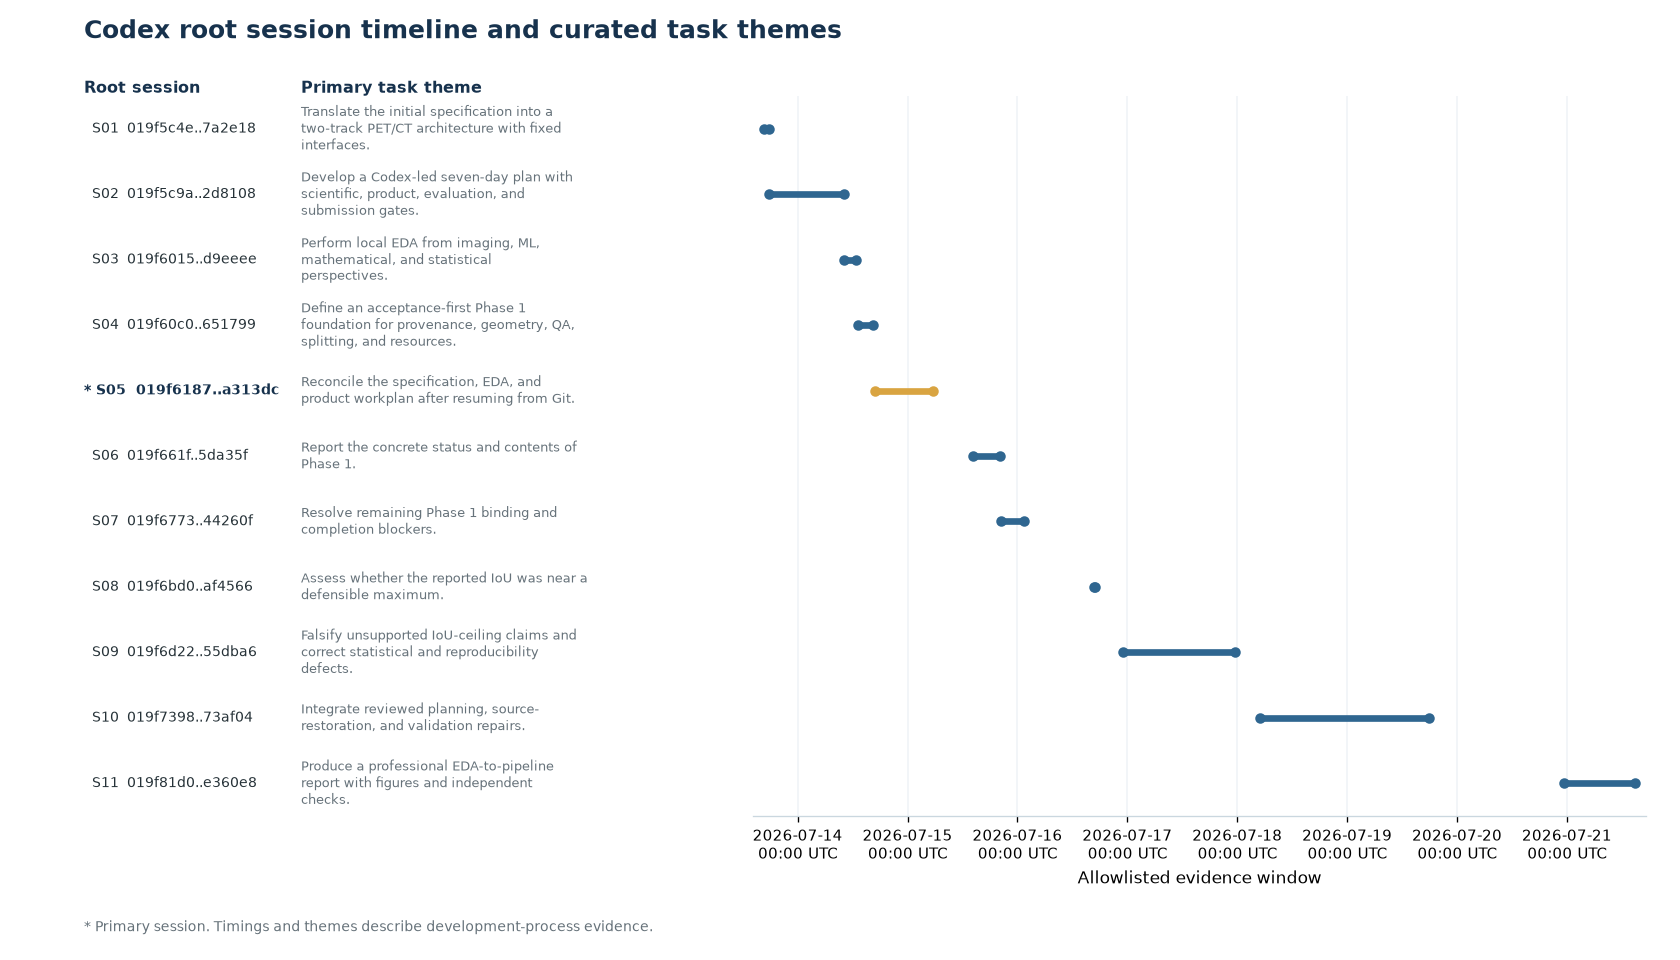
\includegraphics[width=0.99\textwidth]{figures/12_codex_session_timeline.png}
\caption[Codex root-session timeline.]{Codex root-session timeline and task themes. Evidence ID: \evidenceid{SESSION-001}. Population: 11 allowlisted root sessions through the fixed cutoff. Unit: root session and UTC evidence window. S05 is the primary thread. The themes are sanitized receipt fields, not transcript excerpts. This is development-process evidence, not product runtime or scientific-performance evidence.}
\label{fig:codex-session-timeline}
\end{figure}
\clearpage

\begin{figure}[p]
\centering
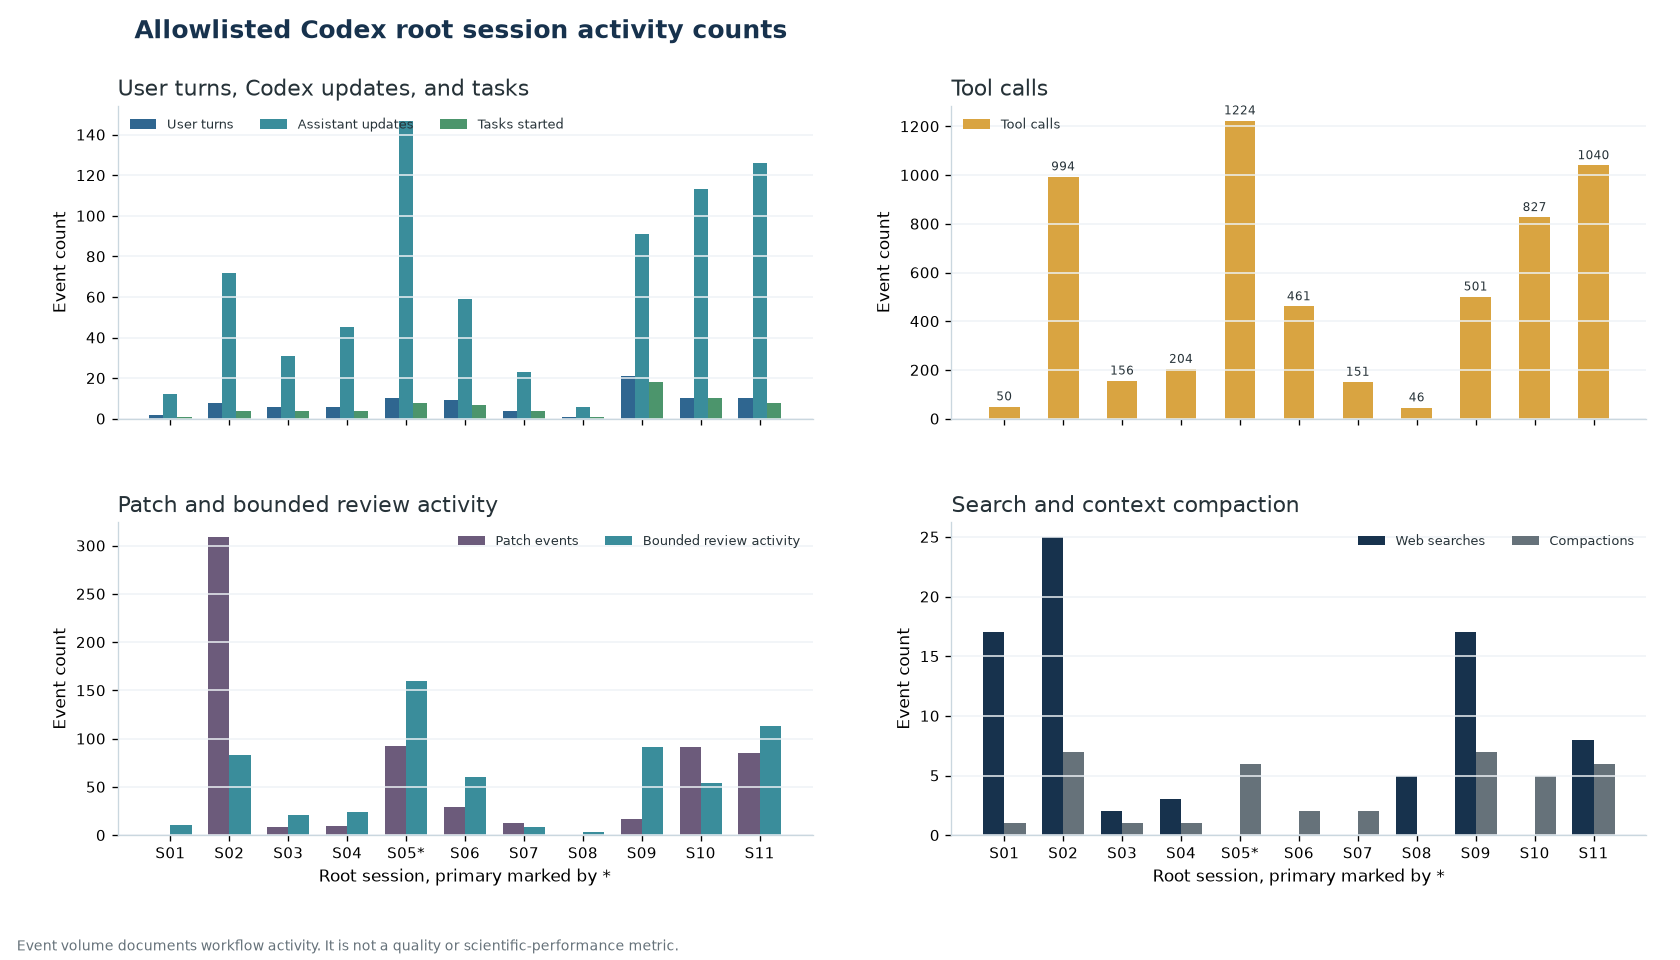
\includegraphics[width=0.99\textwidth]{figures/13_codex_session_activity.png}
\caption[Codex root-session activity counts.]{Allowlisted Codex root-session activity counts. Evidence ID: \evidenceid{SESSION-001}. Population: 11 root sessions through the fixed cutoff. Unit: structural event. Values reproduce the sanitized receipt. Event volume documents workflow activity and is not a quality, labor-time, productivity, authorship-effort, or scientific-performance metric.}
\label{fig:codex-session-activity}
\end{figure}
\clearpage

\subsection{Interpretation boundary for the executed example}

The executed evidence validates that the generated default case can traverse the public product interfaces, preserve measurements in a structured report, reject the tested unsafe claim, isolate case-specific cache queries, fail explicitly on one missing artifact, and emit the complete expected trace. It does not evaluate the learned detector, native-space 3D stitching, physical-space quantification, retrieval quality, scanner behavior, or any clinical endpoint. The generated views are useful demonstration inputs, not examples of confirmed human post-angioplasty abnormalities.

\section{Reproducibility, privacy, and safeguards}

\subsection{Software environment}

The project targets Python 3.13 and uses \texttt{uv} for the locked environment, Ruff for linting and formatting, and pytest for automated tests. Core dependencies include NumPy, SciPy, NiBabel, SimpleITK, PyTorch, Pydantic, MCP, and Streamlit. CPU and offline tests use generated non-patient fixtures. Dataset and GPU tests are marked separately.

The aggregate figure builder reads only the aggregate JSON ledger and writes figures 1 through 8. The product-evidence builder executes generated fixtures in a temporary directory, writes a sanitized JSON receipt, and writes figures 9 through 11. The Codex session-evidence builder reads only the allowlisted structural fields through the fixed cutoff and writes the sanitized receipt and figures 12 and 13. It does not serialize raw messages or local source paths. None of these builders reads medical data or model weights. The report build uses \texttt{pdflatex}, BibTeX, and two final LaTeX passes. The expected commands are listed in Appendix~\ref{app:commands}.

\subsection{Data separation}

Raw medical volumes, subject identifiers, and session manifests remain outside the publication snapshot. Patient-derived per-case results, model weights, and local run outputs are also excluded. The PDF uses no patient or raw medical slice. Its product-view panels come only from the generated default fixture. Figure captions identify each population and independent unit without exposing a subject or workstation path. The retrieval index is also excluded because its earlier corpus was not publication-safe.

\subsection{Determinism and provenance}

The principal deterministic controls are:

\begin{itemize}
  \item subject-grouped split seed 20260713;
  \item primary B2 training seed 20260716;
  \item explicit tensor, crop, model, and checkpoint schema versions;
  \item source-generation seeds and parameter records;
  \item hashes for crop arrays, configurations, checkpoints, and aggregate evidence inputs;
  \item fixed interpolation, connectivity, threshold, and matching policies;
  \item a machine-readable evidence ledger for every public numeric figure.
\end{itemize}

Determinism does not remove bias or validate a scientific assumption. It makes an assumption reproducible and easier to test.

\subsection{Report safeguards}

Measurements must originate from deterministic code. A language component may organize or explain those measurements but must not alter them. Report verification compares structured values to the source, checks expected laterality, requires synthetic status, and screens prohibited claim patterns. The permanent warning is carried in scientific and product artifacts.

The present verifier should be extended. A finite phrase list cannot guarantee claim safety. Future tests should use adversarial paraphrases, omitted qualifiers, changed denominators, unit swaps, laterality changes, structured-null substitutions, and evidence-citation mismatch. Acceptance requires exact numeric fidelity and no unsupported favorable inference.

\section{Limitations}

The following limitations directly constrain interpretation of the results.

\begin{enumerate}
  \item \textbf{No post-intervention human labels.} Training and evaluation use simulated sources in healthy-control backgrounds. The motivating animal study supplies biological context only.
  \item \textbf{Archive label identity remains provisional.} Current public MOOSE documentation supports the label names and codes, but archive files do not independently pin the full versioned mapping.
  \item \textbf{Demographic source discrepancy.} The historical workbook audit and article text differ on the age maximum. This should be reconciled before formal cohort reporting.
  \item \textbf{Legacy reflection geometry.} Current crop bundles use a reflection method that differs from the intended iliac-only, arc-length-paired method.
  \item \textbf{Incomplete factor implementation.} The standard cache did not apply the stored CT shift, and no acquisition-noise model exists. No claim is made for either factor.
  \item \textbf{Baseline mismatch.} The threshold method does not yet implement the complete promotion definition for negative scans and physical component volume.
  \item \textbf{Exploratory center-slice evaluation.} The main result uses 208 center slices from seven subject clusters, not complete scans or a sealed test set.
  \item \textbf{No native-space 3D result.} Slice stitching, native-grid masks, 26-connected components, frozen intersection matching, and 5,000-replicate subject-cluster intervals remain pending.
  \item \textbf{No aggregate quantification-error result.} The standalone 3D quantifier exists, but predicted-mask SUV, volume, extent, and laterality errors were not evaluated in a report-ready aggregate.
  \item \textbf{Product quantification is incomplete.} The learned product path uses a 2D adapter with approximate laterality and structured nulls for unavailable contralateral and physical measurements. It does not yet invoke the complete 3D quantifier.
  \item \textbf{Reference backend is not a model evaluation.} It returns a known synthetic mask and fixed score to test integration.
  \item \textbf{Retrieval evaluation is pending.} The previous index was excluded; a public-only corpus must be rebuilt and reevaluated before retrieval metrics are reported.
  \item \textbf{Historical receipts were not rerun.} Raw-data EDA, crop, and training values in this report are bound to prior artifact hashes and labeled accordingly.
\end{enumerate}

\section{Prioritized completion plan}

\subsection{Gate 1: archive and geometry closure}

Pin the archive-era label map, review fused pelvis overlays locally, implement the intended reflection plane, version the crop schema, and regenerate eligible bundles. Acceptance requires bilateral label identity, finite affines, correct interpolation, reflection involution, side swap, stable centerline pairing, and native-grid round trip.

\subsection{Gate 2: simulator and baseline closure}

Retain the existing source invariants, implement CT-input-only registration stress if it remains in scope, and either build a validated acquisition-noise model or remove that factor from claims. Bring the threshold baseline into the exact negative-scan and physical-component-volume contract. Freeze its score, threshold, and volume rule on validation only.

\subsection{Gate 3: 3D learned evaluation}

Run deterministic sliding center-slice inference, stitch maps into the original PET grid, form 26-connected components, apply frozen matching, and calculate subject-clustered intervals with 5,000 resamples. Select the learned method once on validation, then evaluate the sealed test subjects without retuning. Report raw subject counts beside intervals.

\subsection{Gate 4: quantitative accuracy}

Pass ground-truth and predicted masks through the same standalone 3D quantifier. Report SUVmax error, SUVmean error, volume error, extent error, laterality accuracy, invalid-result counts, and QC strata. Preserve structured nulls. Do not average invalid cases away.

\subsection{Gate 5: product and evidence integration}

Replace the single-slice measurement adapter with native 3D quantification, preserve the completed \scoreterm\ terminology and structured-null behavior, rebuild the evidence index from approved public sources, and reevaluate retrieval. Run end-to-end cases from a clean process, including missing-checkpoint, empty-mask, invalid-denominator, no-evidence, and report-drift failures.

\subsection{Gate 6: external scientific review}

Provide this report, the evidence ledger, the public code snapshot, and the frozen evaluation protocol for review. The most useful review questions are whether the iliac corridor is an adequate method-development anchor, whether the reflection definition is physically defensible, whether the source range is suitable for the stated image-domain question, and whether the final independent unit and uncertainty plan are adequate.

\section{Conclusion}

VascuTrace has progressed from dataset inspection to a functioning method-development stack. It includes physical-grid handling, bilateral crops, synthetic-source insertion, a transparent threshold module, a callable 2.5D Siamese U-Net, standalone deterministic quantification, structured product tools, report generation, and report verification. Aggregate exploratory evidence suggests that the B2 model often overlaps simulated targets on the selected validation center slices, while small radius, high blur, and high background texture remain difficult conditions.

The current evidence is deliberately narrower than the implementation inventory. The principal result is exploratory 2D validation over seven subject clusters. Reflection geometry, baseline definitions, native-space 3D evaluation, sealed testing, product quantification, and public-corpus retrieval evaluation remain open. Those contracts define the next phase of work.

\begin{center}
\fcolorbox{VTRed}{red!4}{\parbox{0.93\textwidth}{\centering\bfseries\warningtext}}
\end{center}

\clearpage
\bibliographystyle{plainnat}
\bibliography{references}

\clearpage
\appendix

\section{Selected evidence ledger entries}
\label{app:ledger}

The complete machine-readable ledger is distributed with the report. Table~\ref{tab:ledger-selected} lists the entries most directly tied to the conclusions.

\begin{longtable}{>{\ttfamily\raggedright\arraybackslash}p{0.13\textwidth} L{0.18\textwidth} L{0.24\textwidth} L{0.24\textwidth}}
\caption{Selected evidence ledger entries. The unit is an evidence record. No row contains case-level data.}\label{tab:ledger-selected}\\
\toprule
ID & Evidence class & Main content & Limitation \\
\midrule
\endfirsthead
\toprule
ID & Evidence class & Main content & Limitation \\
\midrule
\endhead
EDA-001 & Source fact and historical aggregate & 48 subjects, 96 sessions, 960 NIfTI volumes & No raw-data rerun in this publication turn \\
EDA-004 & Source fact and historical header audit & PET and CT grid shapes, spacing, and coverage & Global geometry does not prove local alignment \\
FIT-001 & Historical aggregate under provisional mapping & Bilateral iliac presence, size, and connectivity & Archive-era integer semantics not independently pinned \\
FIT-002 & Historical aggregate and engineering decision & Crop dimensions and six-session receipt & Reflection method mismatch remains \\
SIM-001 & Current implementation observation & Source equation, factors, normalization, and exclusions & No acquisition-noise model; CT shift not applied \\
MODEL-002 & Historical exploratory validation & B2 positive overlap, IoU, component metrics, and negative activation & Seven-cluster center-slice validation only \\
ATLAS-001 & Historical descriptive stratification & Radius, uptake, blur, and two-factor IoU summaries & Small repeated cells; no unclustered inference \\
ATLAS-002 & Historical descriptive stratification & Activation by raw-PET texture-proxy stratum & Proxy is not simulated acquisition noise \\
DEMO-001 & Current generated execution and role summary & Bound product receipt, Figures 9 through 11, structured values, report acceptance, ordered trace, six software checks, and corrected collaboration ownership & Nominal metadata and fixed 0.76 SUV array rule; not physical-space 3D or learned-model evidence \\
SESSION-001 & Sanitized development-process evidence & Eleven root Session IDs, fixed cutoff, recorded model identifiers, structural counts, task themes, public outcomes, and Figures 12 and 13 & Event volume is not quality, labor-time, productivity, authorship-effort, or scientific-performance evidence \\
\bottomrule
\end{longtable}

\section{Report and software verification commands}
\label{app:commands}

The following commands define the publication build and the project-level checks expected before release. A command should be reported as passed only after a fresh run with an exit code of zero. Before building session evidence, \texttt{VASCUTRACE\_CODEX\_SESSION\_INPUT} must point to the approved local Codex session root. Its value is not stored in the public output.

\begin{table}[H]
\centering
\footnotesize
\caption{Publication command matrix. The unit is one command. Dataset and GPU tests remain separate because the default suite must be offline and generated-fixture based.}
\begin{tabularx}{\textwidth}{B{0.25\textwidth} Y}
\toprule
Purpose & Command \\
\midrule
Environment setup & \texttt{uv sync -{}-locked} \\
Build figures & \texttt{uv run python docs/report/scripts/build\_report\_figures.py} \\
Build product evidence & \texttt{uv run python docs/report/scripts/build\_product\_evidence.py} \\
Build session evidence & \texttt{uv run python docs/report/scripts/build\_codex\_session\_evidence.py -{}-session-root "\$VASCUTRACE\_CODEX\_SESSION\_INPUT" -{}-output-root docs/report -{}-cutoff 2026-07-21T14:56:53.784Z -{}-workspace-name VascuTrace\_AI -{}-report-layout} \\
First LaTeX pass & \texttt{cd docs/report \&\& pdflatex -interaction=nonstopmode -halt-on-error} \path{VascuTrace_Technical_Report_2026-07-20.tex} \\
Bibliography & \texttt{cd docs/report \&\& bibtex} \path{VascuTrace_Technical_Report_2026-07-20} \\
Second LaTeX pass & \texttt{cd docs/report \&\& pdflatex -interaction=nonstopmode -halt-on-error} \path{VascuTrace_Technical_Report_2026-07-20.tex} \\
Final LaTeX pass & \texttt{cd docs/report \&\& pdflatex -interaction=nonstopmode -halt-on-error} \path{VascuTrace_Technical_Report_2026-07-20.tex} \\
PDF metadata & \texttt{pdfinfo }\path{docs/report/VascuTrace_Technical_Report_2026-07-20.pdf} \\
PDF text & \texttt{pdftotext }\path{docs/report/VascuTrace_Technical_Report_2026-07-20.pdf}\texttt{ -} \\
Lint & \texttt{uv run ruff check -{}-no-cache .} \\
Format & \texttt{uv run ruff format -{}-check -{}-no-cache .} \\
Offline tests & \texttt{uv run pytest -q -m \textquotesingle{}not local\_data and not gpu\textquotesingle{}} \\
\bottomrule
\end{tabularx}
\end{table}

\section{Claim and terminology matrix}

\begin{table}[H]
\centering
\caption{Approved report vocabulary. The unit is a phrase or claim type.}
\begin{tabularx}{\textwidth}{B{0.24\textwidth} Y Y}
\toprule
Concept & Use & Do not infer \\
\midrule
Source & Simulated vascular-like abnormality or synthetic source & Human lesion or arterial-wall truth \\
Background & Healthy-control PET/CT background & Verified absence of every disease \\
Model output & Uncalibrated \scoreterm & Calibrated clinical estimate \\
Positive result & Target-overlapping prediction on a synthetic validation slice & Clinical sensitivity \\
Negative result & Activation or clean proportion on negative healthy-control slices & Clinical specificity or false-positive rate \\
Blur & Controlled Gaussian image blur & Scanner sensitivity or measured point-spread response \\
Texture & Derived raw-PET texture proxy & Simulated acquisition noise \\
Contralateral side & Within-image reference & Clinically normal tissue \\
\bottomrule
\end{tabularx}
\end{table}

\section{Glossary}

\begin{description}
  \item[Activation] Any predicted component or nonempty prediction on an untouched or negative research input, under the declared rule.
  \item[Abnormality score] An uncalibrated model output used for thresholding or ranking within this research prototype.
  \item[Affine] A $4 \times 4$ mapping from voxel coordinates to physical patient coordinates.
  \item[CT-input registration stress] A controlled transform applied only to the model CT input while PET and labels remain fixed. This was not evaluated in the standard B2 cache.
  \item[Detectability atlas] A table or plot describing image-domain performance across controlled source or background factors.
  \item[IoU] Intersection over union between a predicted binary region and a synthetic target region.
  \item[Native space] The original PET grid and affine in which public spatial outputs and physical measurements should be represented.
  \item[Structured null] A measurement with no numeric value and a typed reason explaining why the measurement is invalid.
  \item[Subject cluster] All visits, slices, and synthetic derivatives belonging to one subject, treated together for splitting and resampling.
\end{description}

\end{document}
